\chapter{Models and Results}
\label{chap:models_and_results}
\section{Technical aspects}
The code repository containing all notebooks, models and results can be found via \newline \url{https://github.com/brianbaert/MscThesis.git} 


All the experiments were done on a single GPU server with the following specifications:
\begin{table}[H]
\centering
\begin{tabular}{|l|l|}
\hline
\textbf{Processors} & 4x Intel(R) Xeon(R) 3-2286G CPU @ 4.00GHz \\
\hline
\textbf{Operating System} & Microsoft Windows Server 2022 Datacenter \\
\hline
\textbf{GPU} & NVIDIA RTX A4500 (20GB) \\
\hline
\textbf{RAM} & 32 GB \\
\hline
\end{tabular}
\label{tbl:specifications}
\caption{Server specifications}
\end{table}

\section{Data description}
\label{sec-DataDesc}
\subsection{Gravity Spy dataset}
The dataset includes 23 different types of glitches represented by time-frequency spectrograms. These glitches have been detected using the Omicron trigger pipeline \citep{robinet2020omicron}, which applies specific criteria such as identifying real-time events with a \acrshort{snr} above 7.5 and a peak frequency ranging from $10 Hz$ to $2048 Hz$. Subsequently, the strain data is transformed into time-frequency spectrograms using the Q-transform process \citep{chatterji2004multiresolution}, these spectrograms are also known as Omega scans.
Gravity Spy produces four spectrograms for every detected glitch, utilizing different time windows: 0.5s, 1.0s, 2.0s, and 4.0s. An illustration of a "Koi Fish" anomaly is depicted in figure \ref{fig:koifish}, while an instance of a "Whistle" anomaly is displayed in figure \ref{fig:whistle}.
\begin{figure}[H]
    \centering
    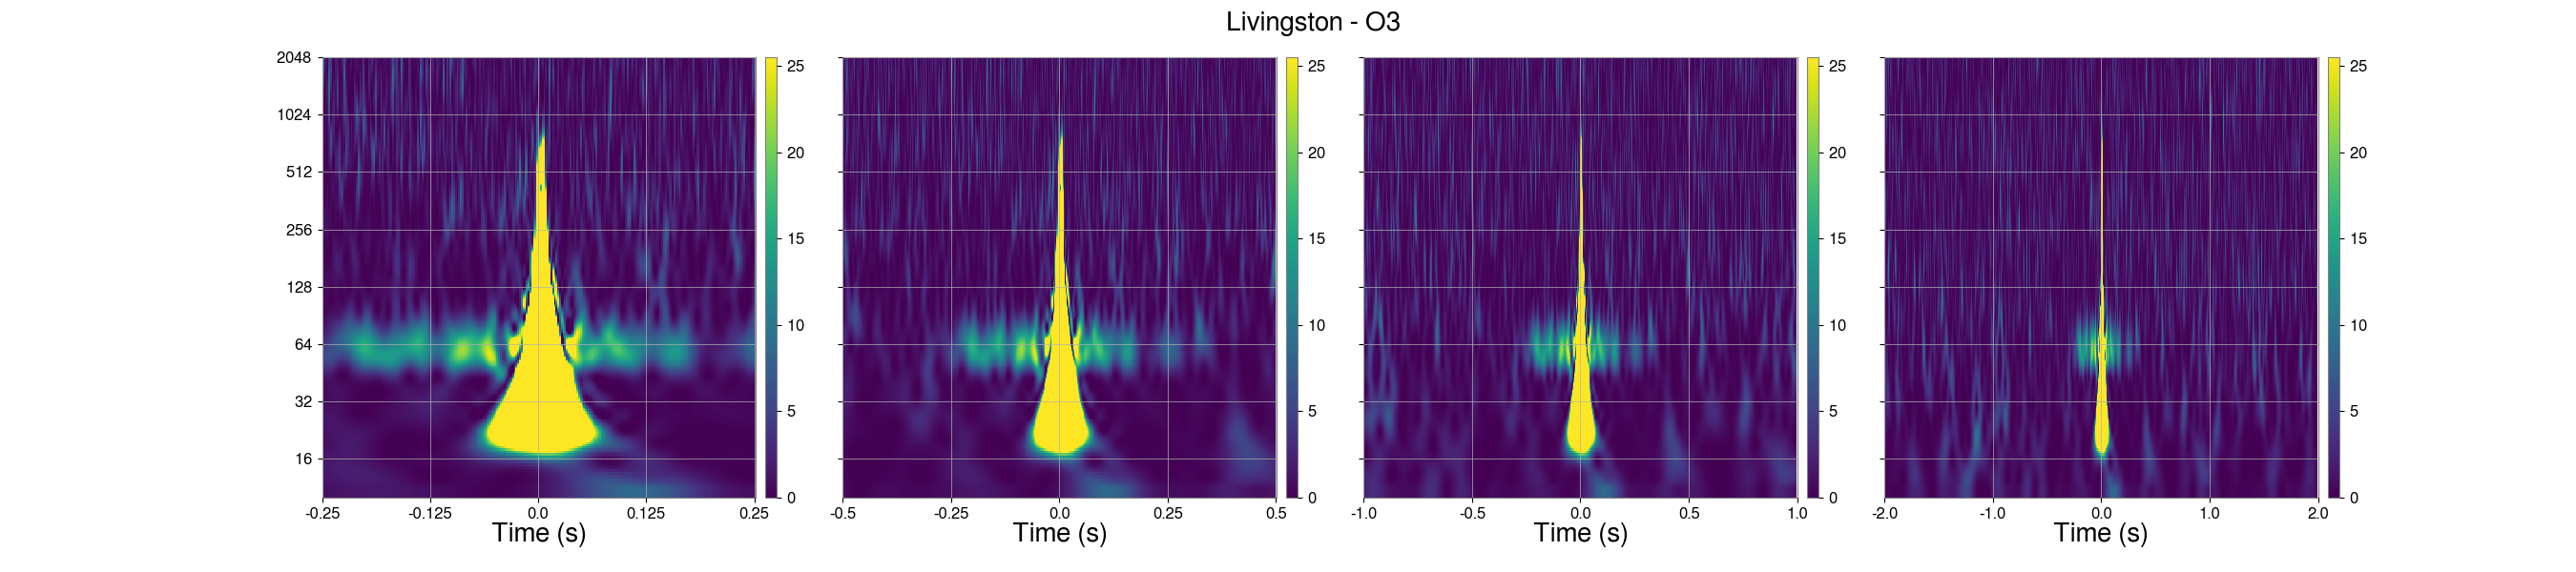
\includegraphics[width=0.9\textwidth]{Images/koi_fish_1250427024.302.png}
    \caption{Spectrogram example of a Koi Fish glitch with four time windows (0.5s, 1.0s, 2.0s an 4.0s}
    \label{fig:koifish}
\end{figure}
\begin{figure}[H]
    \centering
    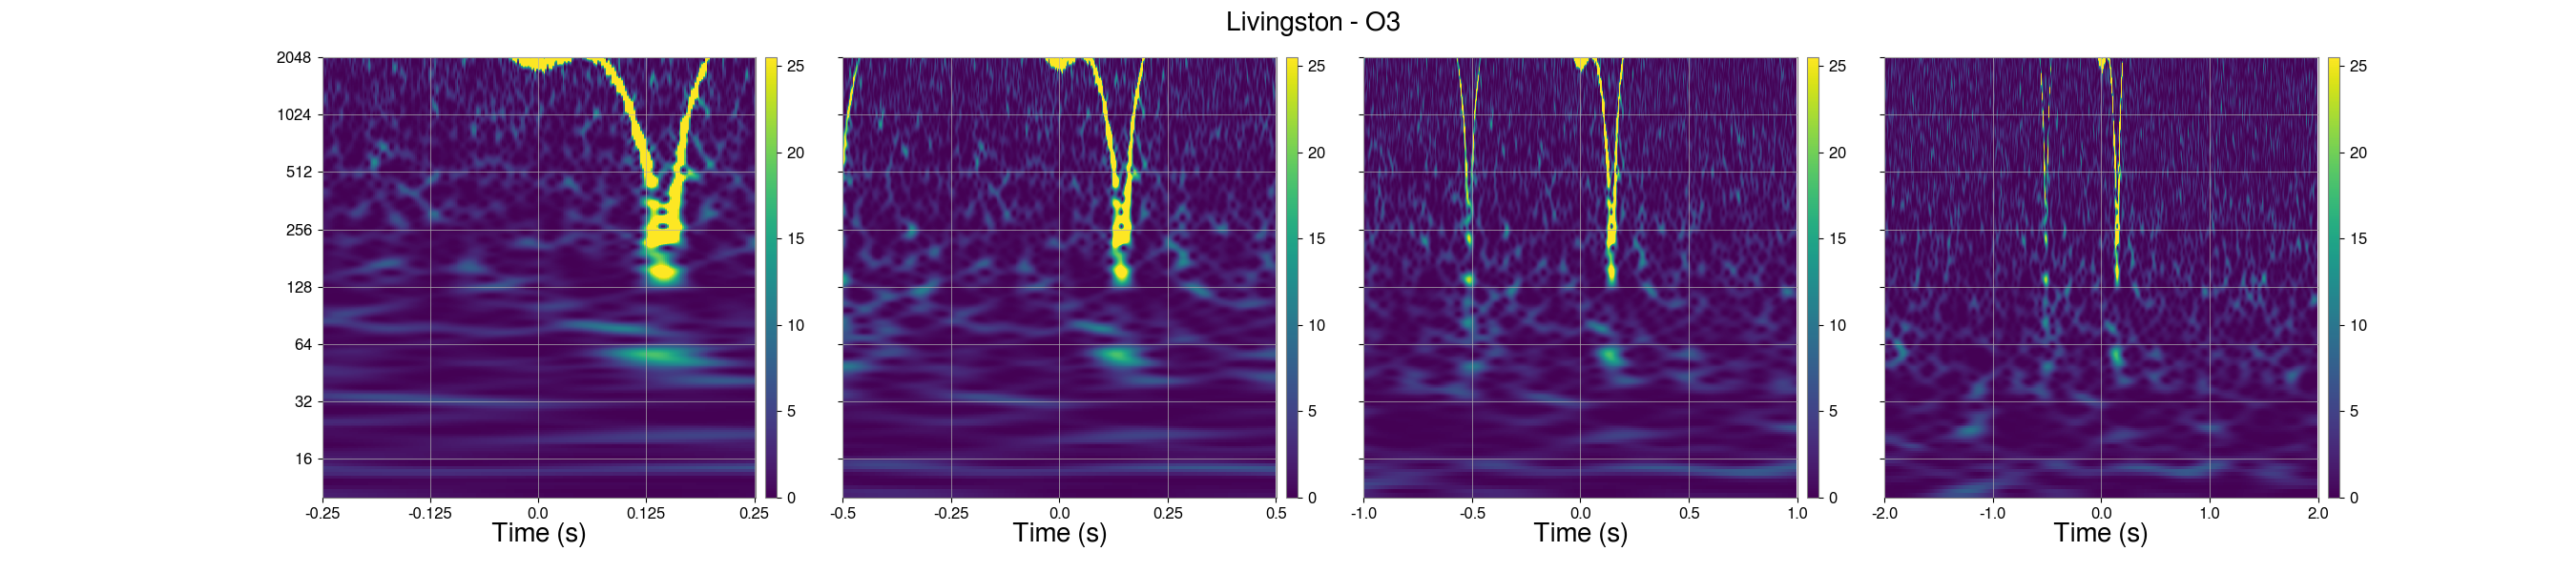
\includegraphics[width=0.9\textwidth]{Images/whistle_1239025005.518.png}
    \caption{Spectrogram example of a Whistle glitch with four time windows (0.5s, 1.0s, 2.0s an 4.0s}
    \label{fig:whistle}
\end{figure}
The class names were established collaboratively by LIGO and citizen scientists. However, there may be a noisy-label problem in the ground truth, as some misclassifications of glitches occurred by both the classifier and volunteers. Hence, it is essential to focus on glitches with a confidence score exceeding 0.9. The dataset shows an imbalance, with O3a having mostly Fast scattering and Tomte glitches, whereas O3b contains mainly Scattered light or Fast scattering glitches. Preliminary results (obtained from LigoDV-Web\footnote{https://ldvw.ligo.caltech.edu/ldvw/gspySearch}) of O4a are mainly Low Frequency burst (45,8\%) and Low Frequency lines (33,1\%) . 

\subsection{O3 Auxiliary Channel data}
As described on the GWOSC\footnote{https://gwosc.org/O3/auxiliary/} website, the O3 auxiliary channel dataset includes channels (more than 200 000 per detector) that were used to create data quality flags, subtract instrumental noise from the strain data and measure the amount of correlated noise between the \acrshort{gw} detectors. 
Data quality flags play a crucial role in the O3 auxiliary channel data, serving to eliminate time periods where data integrity may be compromised by instrument-related or environmental interference. At times, an auxiliary channel may capture extraneous noise sources such as scattered light or power frequency variations, enabling \acrshort{ligo} to enhance the accuracy of strain data by removing such noise components. Conversely, an auxiliary channel can also serve as an indicator of detector glitches, signaling instances of malfunction to analysts for data reliability assessment. Nonetheless, this approach may be flawed if auxiliary channels inadvertently detect disturbances in the gravitational wave channel, leading to the simultaneous appearance of an astrophysical signal in both channels. Channels that detect heightened power levels from the gravitational wave channel are labeled as "unsafe" for vetoing purposes, while those unaffected by this interference are deemed "safe." Vetoing of gravitational wave candidates relies solely on data from "safe" channels. 

Each channel is identified by a name following the format \verb|[IFO]:[SYSTEM]-[NAME]| , where \verb|[IFO]|  denotes the instrument (L1, H1, ...), \verb|[SYSTEM]|  specifies the subsystem (PSL, IMC, TCS, PEM, ...), and \verb|[NAME]|  provides a description of the channel. The dataset available on the GWOSC website comprises 40 channels from the collective \acrshort{ligo} detectors (Hanford, Livingston) that were utilized in the O3 analysis. The dataset has a total size of 13 TB, the full channel list can be found via the \acrshort{ligo} git repository\footnote{https://git.ligo.org/gwosc/}
\citep{GravitySpy20Wiki}

\section{Model}
\subsection{Model design and parameter choices for RQ1}
\label{model_RQ1}
The \verb|MultiViewColorNet_resnet18| architecture is a PyTorch model extending the \newline \verb|nn.Module| class. It is designed for a multi-class classification task. 
\begin{figure}[H]
    \centering
    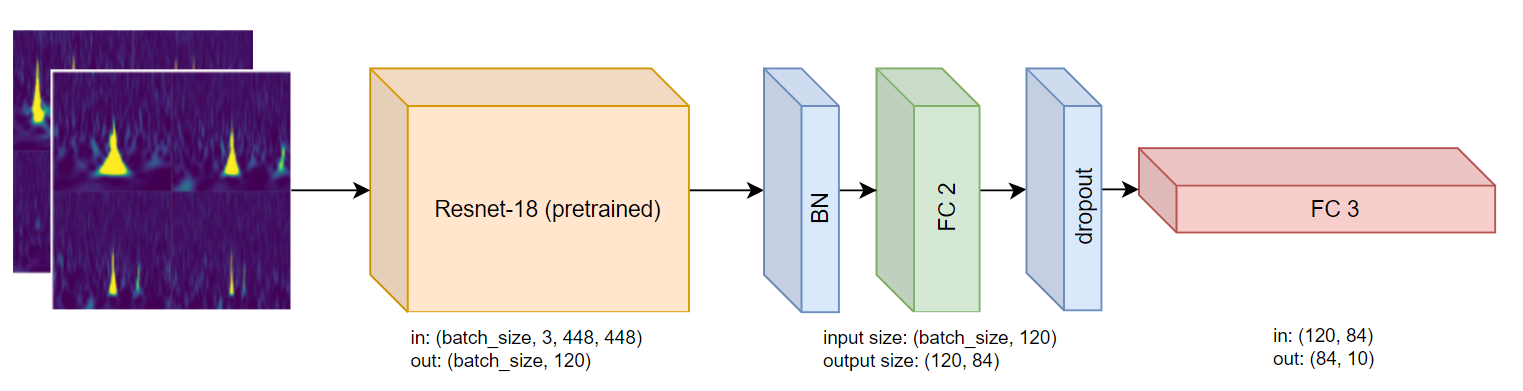
\includegraphics[width=1.0\textwidth]{Images/SlimResnet18_Multiview_CL.png}
    \caption{MultiviewColorNet\_SlimResnet18}
    \label{fig:slimresnet18_multiview}
\end{figure}
The full PyTorch implementation can be found in Appendix \ref{appendix1}, in short the implementation consists of:
\begin{itemize}
    \item A pre-trained ResNet-18 model is loaded into \verb|self.resnet|. The weights are set to 'DEFAULT' (pre-trained on ImageNet). 
    \item The kernel size of the first convolutional layer in the ResNet model adapted to (7x7), this is a common practice in ResNet-based architectures \citep{tomen2021spectral} and has been succesfull in medical image classification on imbalanced datasets \citep{mursalim2021multi}.
    \item All parameters in the ResNet model are unfrozen, allowing them to be updated during training. 
    \item The last layer of the ResNet model, a fully connected layer, is replaced with a new linear layer that has 120 output features. 
    \item Two additional fully connected layers (\verb|self.fc2| and \verb|self.fc3|) are added, with the final layer outputting a number of features equal to \verb|num_classes|.
    \item A dropout layer (\verb|self.dropout|) with a dropout probability of 0.3 is added to help prevent overfitting (according to \citep{park2017analysis} 0.3 is a good value for more complex CNN's like ResNet). 
    \item A batch normalization layer (\verb|self.bn|) is added to normalize the activations of the neurons in the network. 
\end{itemize}

The train dataset contains a balanced random selection of spectrograms from 10 glitch classes ('Blip', 'Blip\_Low\_Frequency', 'Extremely\_Loud', 'Fast\_Scattering', 'Koi\_Fish', \\
'Low\_Frequency\_Burst', 'Low\_Frequency\_Lines', 'Scattered\_Light', 'Tomte', 'Whistle')
(each datapoint consists of a 0.5, 1.0, 2.0 and 4.0 second view of the glitch). 

The spectrograms containing glitches are fused via a custom PyTorch DataLoader extending the ImageFolder class. It concatenates the views into a single image of size 448 by 448 (see Figure \ref{fig:fused_image_tomte} for an example), allowing a model to learn from all views simultaneously. This is particularly useful because different views of a glitch can provide different insights. The final image and its label are returned. 

\begin{figure}[H]
    \centering
    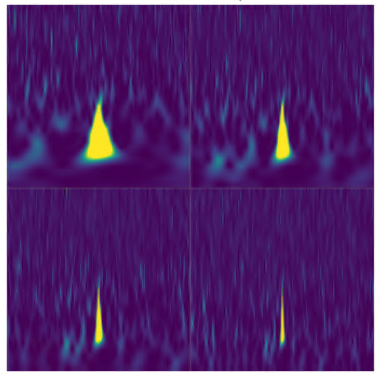
\includegraphics[width=0.5\textwidth]{Images/FusedImage_Tomte.png}
    \caption{Example of a fused image (glitch type 'Tomte').}
    \label{fig:fused_image_tomte}
\end{figure}

The Avalanche \ref{sec:avalanche} New Classes benchmark (\verb|nc_benchmark|) is used because it is specifically designed for creating benchmarks in a "New Classes" continual learning scenario, where each experience introduces new classes that were not present in the previous experiences. Here we opt for 5 experiences (2 classes per experience). \\


The optimizer for the majority of experiments is the \verb|AdamW| optimizer, a variant of the Adam optimizer including weight decay. It is often preferred over standard Adam because it handles weight decay in a more principled manner, leading to better generalization on some tasks \citep{loshchilov2019decoupled}. The learning rate is set to 0.001 and weight decay to 0.00001. These are common hyperparameter choices for AdamW. \\



The criterion used for the experiments is CrossEntropyLoss, a common choice for multi-class classification tasks. This loss function combines LogSoftmax\footnote{Applies the $\log (\text{Softmax} (x))$ function to an input Tensor. \citep{miranda2017softmax}} and NLLLoss\footnote{Negative Log Likelihood Loss \citep{miranda2017softmax}} in one single class, making it suitable for training a classification problem with more than 2 classes. 
\newpage
\subsection{Model design and parameter choices for RQ2}
\label{model_rq2}
The \verb|FractalDimensionConvNet| architecture is a PyTorch model extending the \newline \verb|nn.Module| class and uses a combination of convolutional layers, batch normalization, dropout and fully connected layers. It is designed for a multi-class classification task. 
\begin{figure}[H]
    \centering
    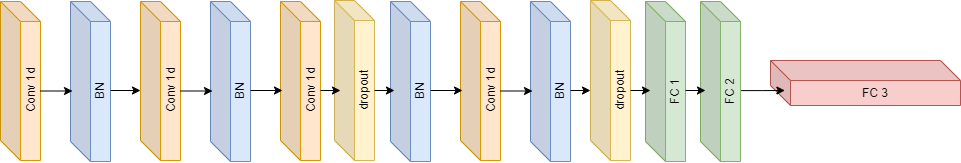
\includegraphics[width=1.0\textwidth]{Grad Assignment/Images/FD_architecture.drawio.png}
    \caption{FractalDimensionConvNet}
    \label{fig:FractalDimensionConvNet}
\end{figure}
The full PyTorch implementation can be found in Appendix \ref{appendix3}, in short the implementation consists of:
\begin{itemize}
    \item Four pairs of 1-dimensional convolutional layers (\verb|nn.Conv1d|) are used to process the fractal dimension data into a 1-dimensional format. 
    \item Fully connected Layers are added to flatten the output and output a three-class prediction. 
    \item Two dropout layers (\verb|self.dropout|) with a dropout probability of 0.1 and 0.3 are added to help prevent overfitting. 
    \item Four batch normalization layers (\verb|self.bn|) are added to normalize the activations of the neurons in the network. 
    \item The model uses the SELU (Scaled Exponential Linear Unit) activation function after each convolutional and the first fully connected layer, which can lead to self-normalizing neural networks \citep{rasamoelina2020review, kiliccarslan2021overview}. The second fully connected layer users the ReLU activation function. 
\end{itemize}

The train dataset contains a balanced (896 entries for each of the three glitch categories) selection of 2688 records where each record contains fractal dimension calculations on 50 auxiliary channels from 3 glitch classes ('Whistle', 'Tomte', 'Scattered\_Light'). Each channel has 56 fractal dimension calculations. The dataset selection is based on the study by \citep{laguarta2023detection}.

An example visualisation is show in Figure \ref{fig:FD_visualisation}
\begin{figure}[ht]
    \centering
    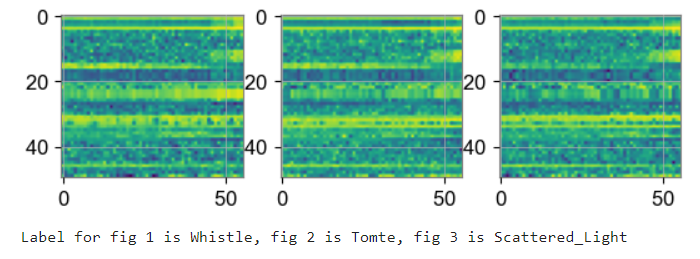
\includegraphics[width=0.5\textwidth]{Grad Assignment/Images/FD_visualisation_50channels.png}
    \caption{Example visualisations of FD matrices with 50 channels. Left = 'Whistle', Middle = 'Tomte' and right = 'Scattered\_Light'}
    \label{fig:FD_visualisation}
\end{figure}

The optimizer for the majority of experiments is the \verb|AdamW| optimizer. The learning rate is set to 0.001 and weight decay to 0.00001. Finally, the criterion used for the experiments is CrossEntropyLoss just as in \ref{subsubsec:RQ1_naive_baseline}. 
\newpage
\subsection{Model design and parameter choices for RQ3}
\label{model_RQ3}
The \verb|MultiModalNet| architecture is a PyTorch model extending the \newline \verb|nn.Module| class and uses a combination of the \verb|MultiViewColorNet| architecture of RQ1 \ref{model_RQ1} and the \verb|FractalDimensionConvNet| of RQ2 \ref{model_rq2}. 
The outputs of both models are concatenated and send through a fully connected linear layer mapping the outputs to the final output classes. 

\begin{figure}[H]
    \centering
    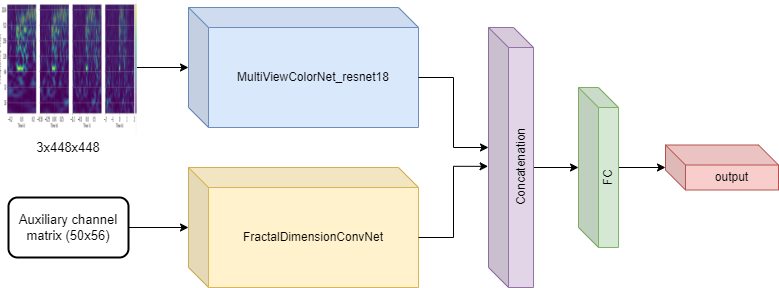
\includegraphics[width=1.0\textwidth]{Images/MultiModal_architecture.drawio.png}
    \caption{MultiModalNet architecture}
    \label{fig:MultiModal_architecture}
\end{figure}

The model uses the \verb|CrossEntropyLoss| function designed for multiclass classification and the \verb|AdamW| optimizer. The learning rate is set to the default value $0.001$ and weight decay to $0.00001$.

Due to the fact that the \acrshort{cl} package \verb|Avalanche| \citep{lomonaco2021avalanche} does not provide native Multimodal support, the experimentation is limited to a basic Multimodal pytorch training loop. 
\newpage
\section{Results}
\subsection{RQ1}
\label{subsec:RQ1}
Each of the strategies are trained for 100 epochs on every task (of distinguishing between two glitch categories). The order in which the classes are fed is kept the same over all strategies (1 = \{Koi\_Fish; Low\_Frequency\_Burst\}, 2 = \{ Tomte; Extremely\_Loud \}, 3 = \{ Whistle; Fast\_Scattering \}, 4 = \{ Blip\_Low\_Frequency ; Scattered\_Light \} and 5 = \{ Blip; Fast\_Scattering \} )

\subsubsection{Naive CL strategy (baseline)}
\label{subsubsec:RQ1_naive_baseline}
As baseline we use the \acrshort{cl} stategy 'Naive'. This is the simplest form of \acrshort{cl}, where the model is trained on each task (in our setting we have 5 tasks (experiences) consisting of two classes per task) in sequence without any explicit mechanism to mitigate catastrophic forgetting. However, because early runs of this model suffered from extreme recency bias, the strategy is augmented with a couple of plugins to improve its performance: 
\begin{itemize}
    \item \verb|ReplayPlugin|: this plugin implements experience replay, a common technique to mitigate catastrophic forgetting. It stores a subset of the training data and interleaves training on the current task with training on the stored data. The memory size is set to twice the size of the training set, meaning it can store two complete copies of the training set. 
    \item \verb|EarlyStoppingPlugin|: This plugin implements early stopping, and thus prevents overfitting. 
\end{itemize}
During training we keep track of the weight distribution changes via violin plots. 
After the first 100 epochs training on differentiating the classes from experience 0 to 4 we get: 
\begin{center}
\begin{tabular}{cc}
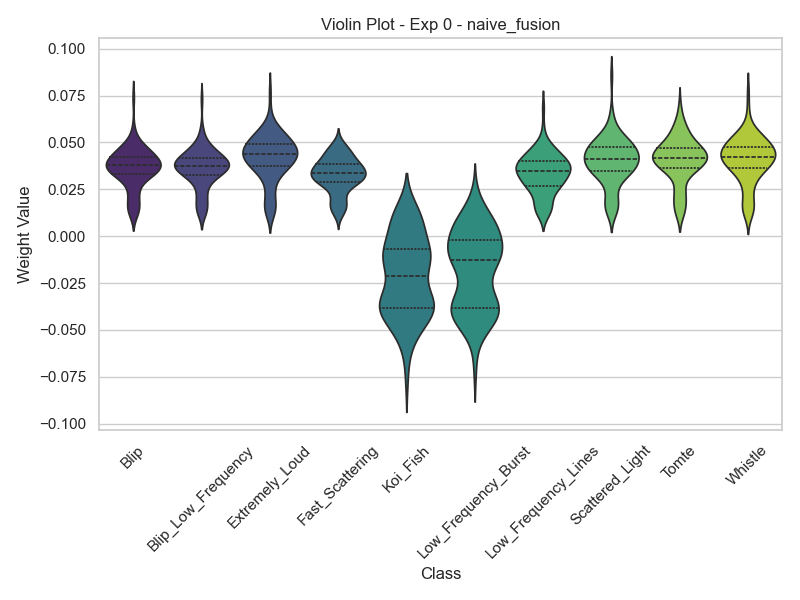
\includegraphics[width=0.4\textwidth]{Images/naive_fusion_exp_0.png} & 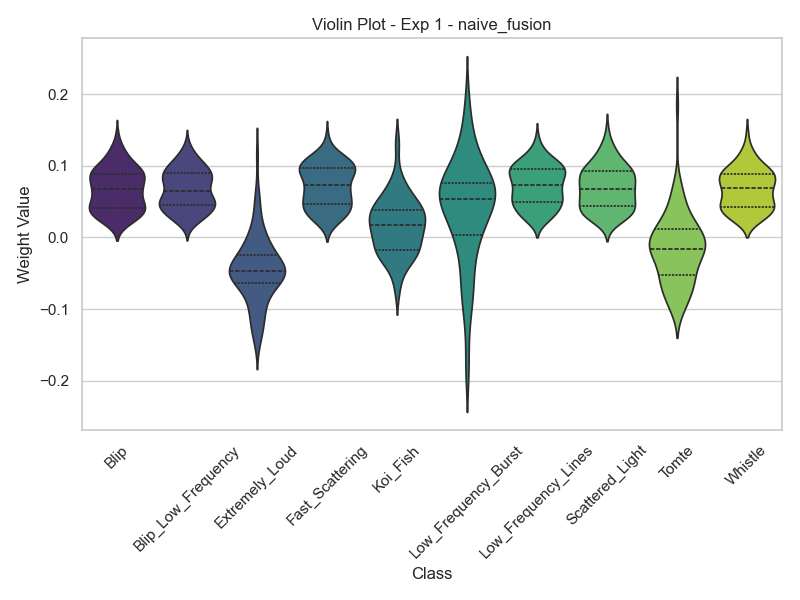
\includegraphics[width=0.4\textwidth]{Images/naive_fusion_exp_1.png} \\
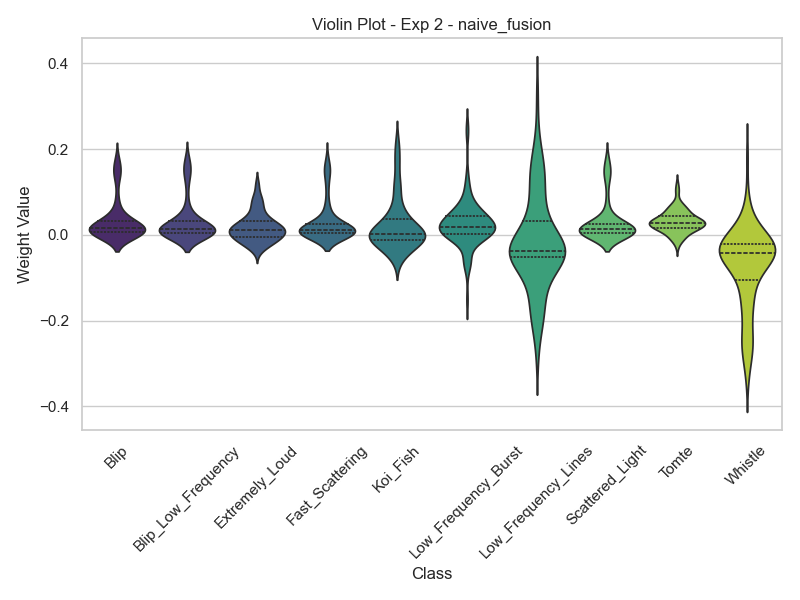
\includegraphics[width=0.4\textwidth]{Images/naive_fusion_exp_2.png} & 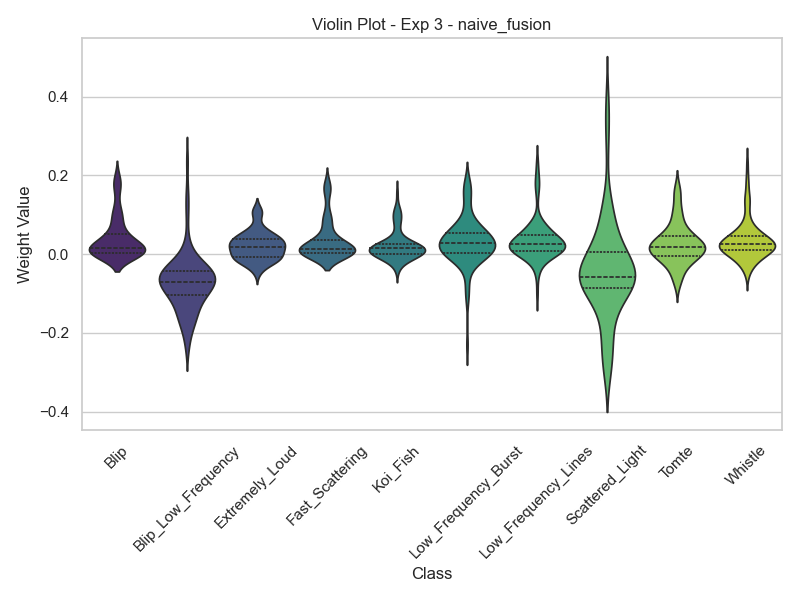
\includegraphics[width=0.4\textwidth]{Images/naive_fusion_exp_3.png}
\end{tabular}
\end{center}
\begin{center}
    \begin{tabular}{c|c}
         \multicolumn{2}{c}{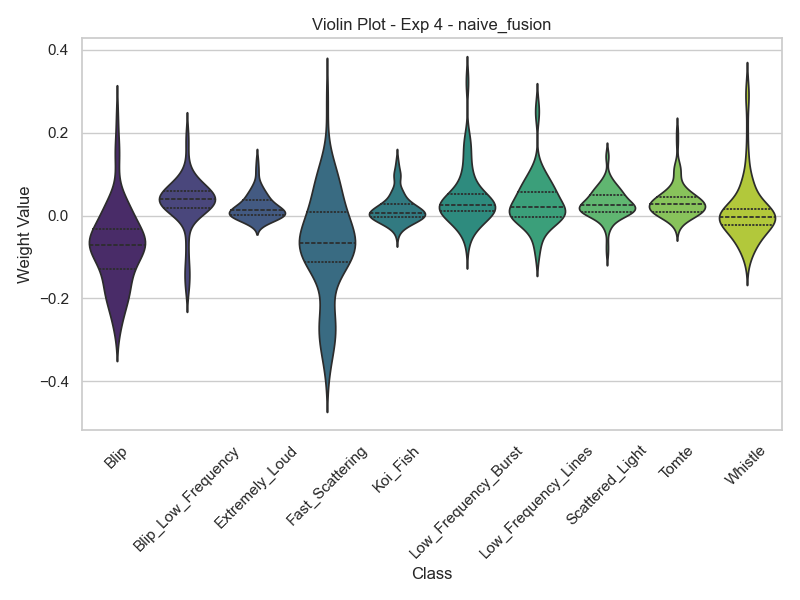
\includegraphics[width=0.4\textwidth]{Images/naive_fusion_exp_4.png}}
    \end{tabular}
\end{center}
For each experience, the weights for the Softmax classification corresponding to the classes in that experience in the fully connected layer are adjusted more than for the other classes. The median shift and distribution shape of the violin body illustrate this. 

From the Confusion Matrix as shown in Figure \ref{fig:cm_f1_naive_baseline}-(a) we find that the overall accuracy is $81.8 \%$. Some glitch classes like 'Whistle' and 'Frequency\_Lines' have perfect accuracy, whilst others like 'Blip\_Low\_Frequency' and 'Tomte' suffer from a lot of False Negatives, on the other hand 'Blip' suffers from a lot of False Positives. 

\begin{figure}[ht]
\centering
\begin{subfigure}
  \centering
  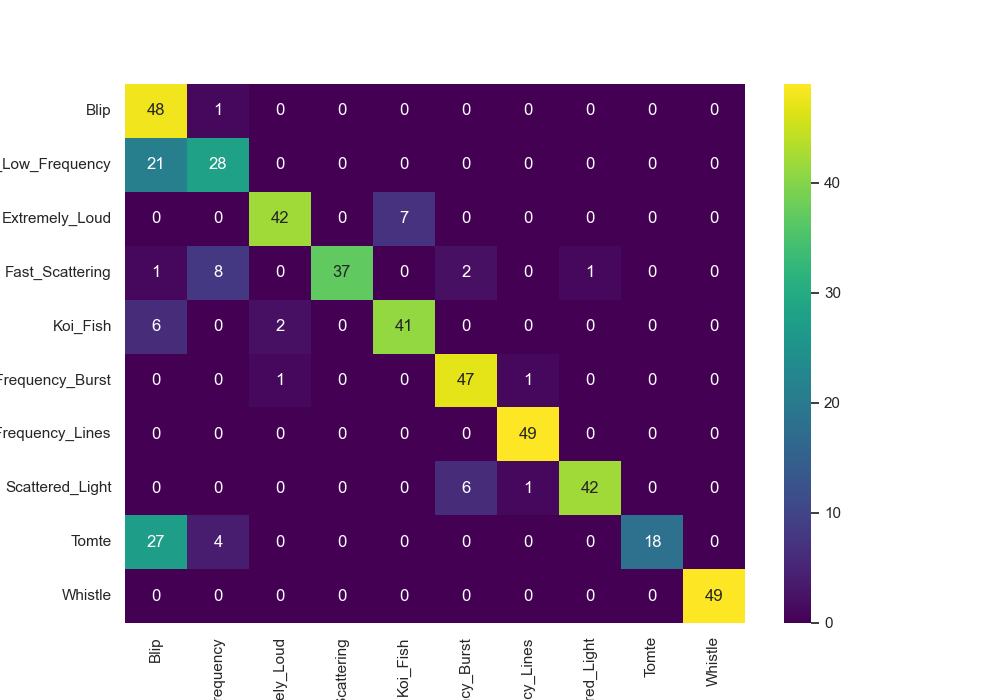
\includegraphics[width=0.49\textwidth]{Grad Assignment/Images/cm_MultiView_Naive_100epochs.png}  
  \label{fig:sub-first1}
\end{subfigure}
\begin{subfigure}
  \centering
  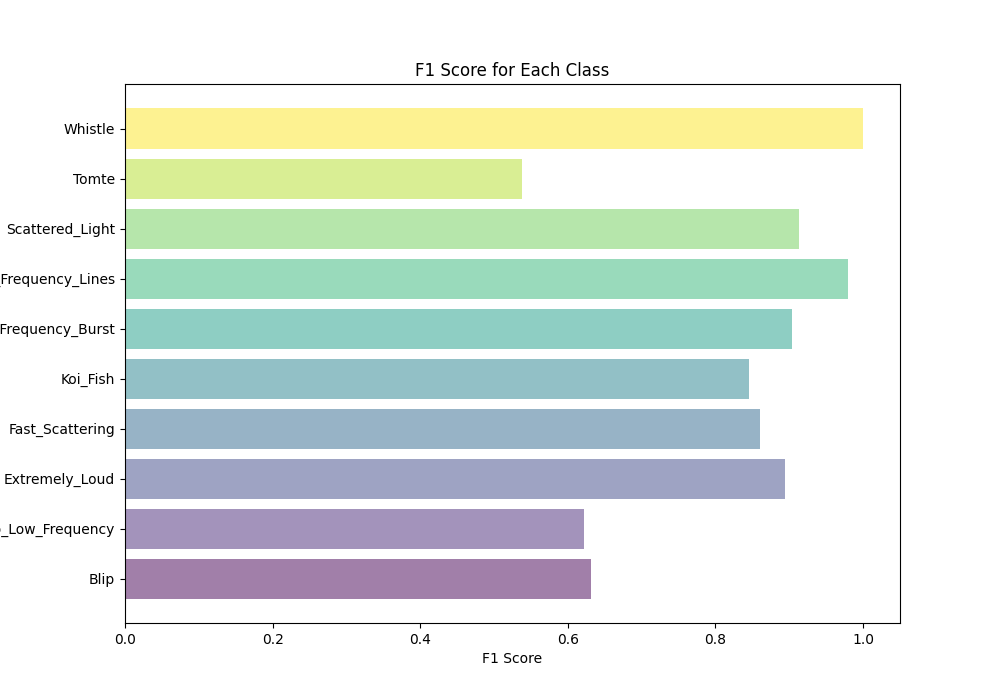
\includegraphics[width=0.49\textwidth]{Grad Assignment/Images/f1_MultiView_Naive_100epochs.png}  
  \label{fig:sub-second1}
\end{subfigure}
\caption{Confusion matrix and f1 plot for Naive baseline}
\label{fig:cm_f1_naive_baseline}
\end{figure}

We investigate the \acrshort{tsne} and \acrshort{umap} representations\footnote{UMAP tends to better preserve global structure compared to t-SNE, it strikes a balance between global and local structure. \citep{mcinnes2018umap}}, 
The t-SNE visualization as shown in Figure \ref{fig:tSNE_Naive} illustrates a clustering of glitch classes in 2D space. The separation of most glitch categories like 'Whistle' and 'Scattered\_Light' is apparent. But the overlap of the Glitch categories 'Blip', 'Blip\_Low\_Frequency' and 'Tomte' could proof problematic in producing False positives for one of the three classes.
A similar interpretation can be made from Figure \ref{fig:umap_Naive}. Here 'Koi\_Fish' and 'Extremely\_Loud' as well as 'Blip', 'Blip\_Low\_Frequency' and 'Tomte' are relatively close to eachother, suggesting shared global features. 

\newpage
\begin{figure}[ht]
\centering
\begin{subfigure}
  \centering
    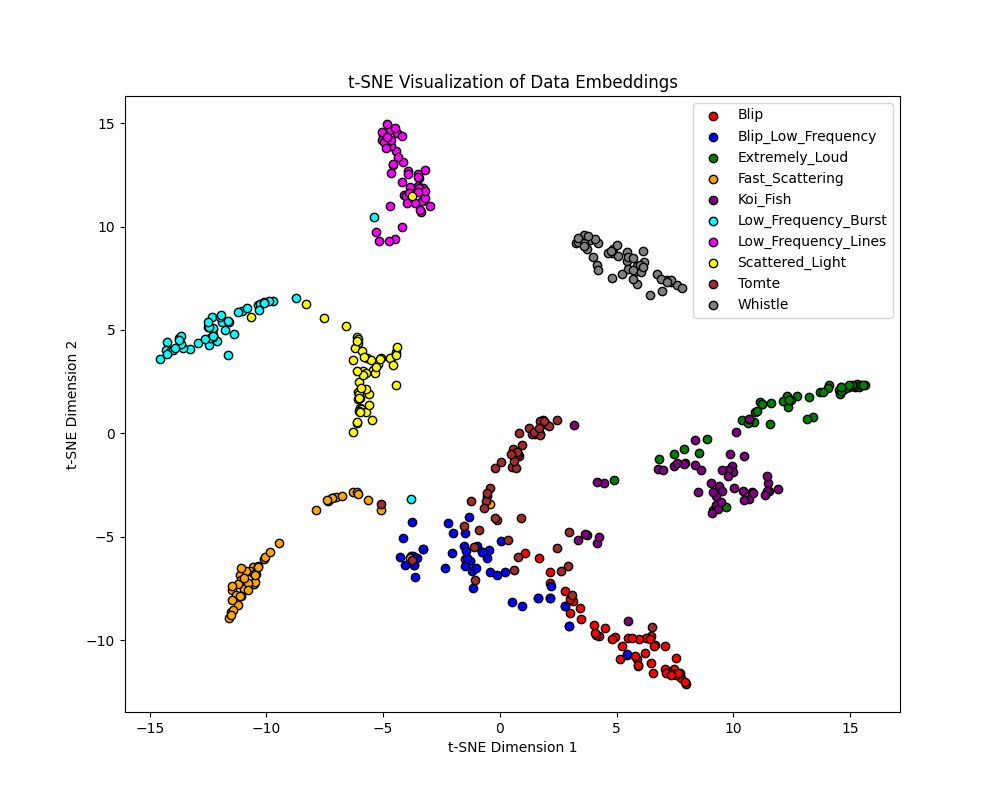
\includegraphics[width=0.6\textwidth]{Images/tSNE_MultiView_Naive_testset_100epochs.png}
    \caption{t-SNE visualization Naive strategy}
    \label{fig:tSNE_Naive}
\end{subfigure}
\begin{subfigure}
  \centering
    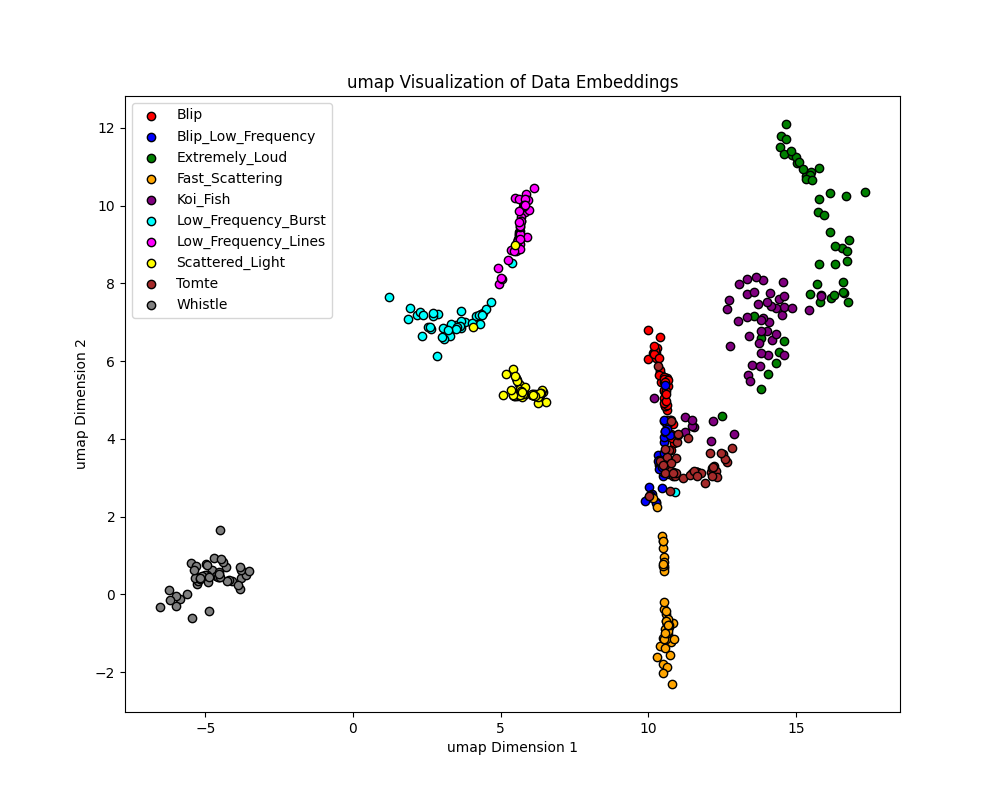
\includegraphics[width=0.6\textwidth]{Images/umap_MultiView_Naive_testset_100epochs.png}
    \caption{UMAP visualization Naive strategy}
    \label{fig:umap_Naive}
\end{subfigure}
\end{figure}

The images of the Saliency Mapping in Figure \ref{fig:saliency_naive_baseline} confirm some of the misclassifications we already concluded from the Confusion Matrix. Specifically on row 2 and row 3 we see the 'Blip\_Low\_Frequency' misclassified as a 'Blip'. It is clear that the shape of these two are very similar. 
Because 'Blip' is provided in the last experience, the recency bias favors this category. Presumably if the 'Blip\_Low\_Frequency' was used in the last experience, the results would be mirrored. 

\begin{figure}
    \centering
    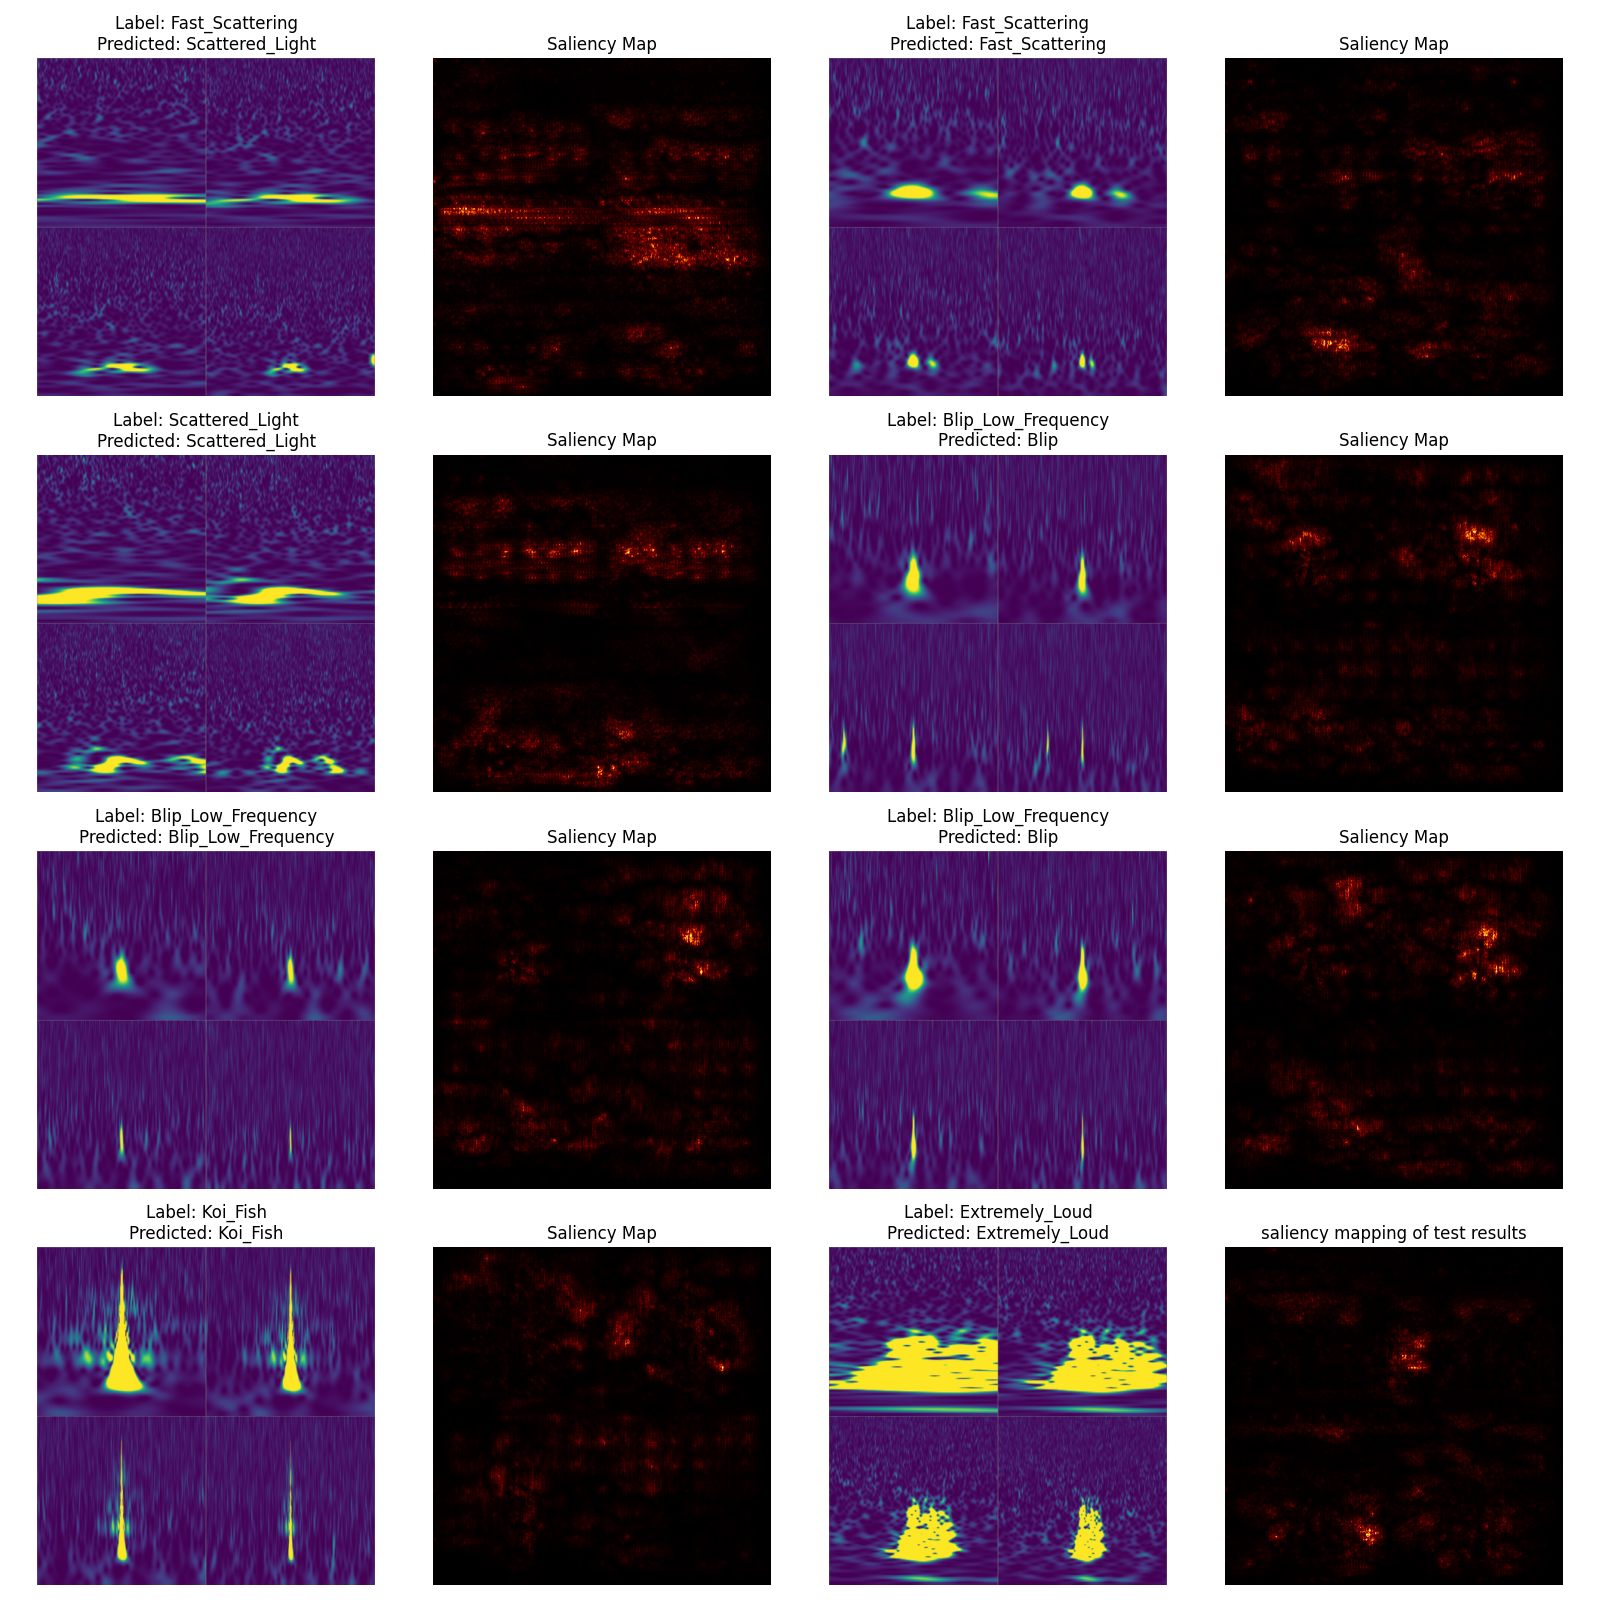
\includegraphics[width=0.95\textwidth]{Grad Assignment/Images/SaliencyMapping_Naive_MultiView_100epochs.png}
    \caption{Saliency Mapping of Naive baseline}
    \label{fig:saliency_naive_baseline}
\end{figure}

\newpage
\subsubsection{LwF strategy}
\label{subsubsec:RQ1_LWF}
A first \acrshort{cl} strategy addressing catastrophic forgetting is called \acrfull{lwf}. The model is trained, just as in the naive baseline, on five distinct tasks that contain two classes per experience. 
The hyperparameter choices are: 
\begin{itemize}
    \item \verb|alpha=0.25|: $\alpha$ controls the balance between the loss on the new task and the distillation loss used to retain knowledge from old tasks. A value of 0.25 is a common choice based on the paper by \citep{oren2021defense}. 
    \item \verb|temperature=2.0|: $\tau$ controls the "softness" of the logits during knowledge distillation. A higher $\tau$ leads to softer targets, encouraging the network to learn a more generalizable representation that benefits both old and new tasks. 
\end{itemize}

The strategy is augmented with the same \verb|ReplayPlugin|. 
Early stopping is not inherently supported by \acrshort{lwf} and thus not applied. 

Changes in weight distribution are also tracked. A similar behavior can be found. For illustrative purposes we only show the violin plots after the first and the last experience. 

\begin{figure}[ht]
\centering
\begin{subfigure}
  \centering
  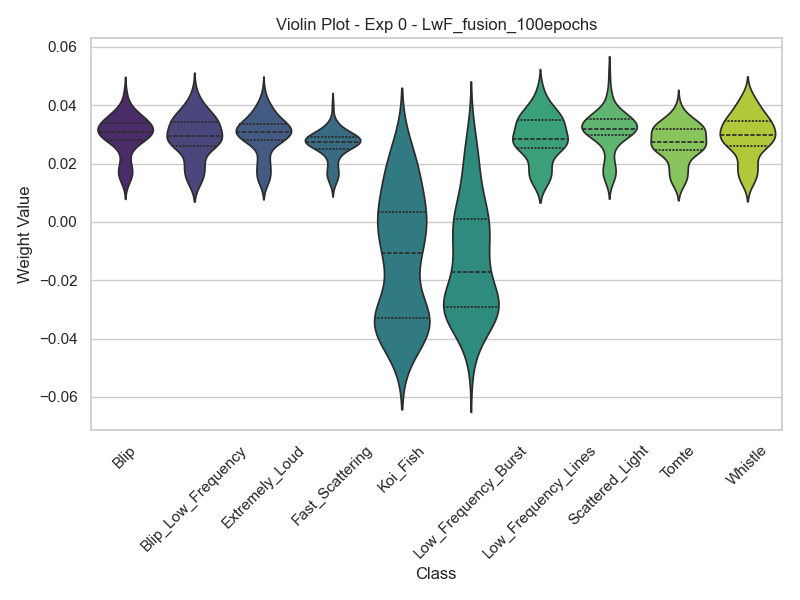
\includegraphics[width=0.4\textwidth]{Grad Assignment/Images/LwF_fusion_100epochs_exp_0.png}  
  \label{fig:lwf_violin_exp_0}
\end{subfigure}
\begin{subfigure}
  \centering
  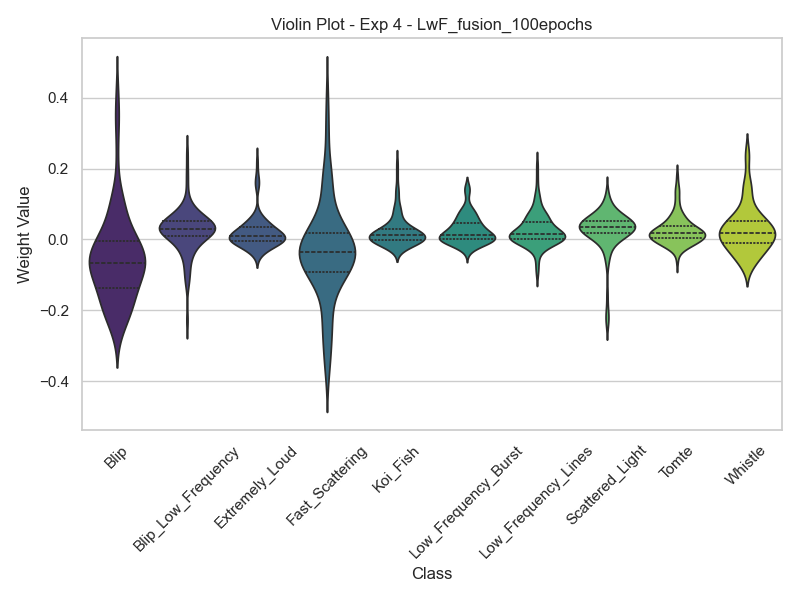
\includegraphics[width=0.4\textwidth]{Grad Assignment/Images/LwF_fusion_100epochs_exp_4.png}  
  \label{fig:lwf_violin_exp_4}
\end{subfigure}
\caption{Weight distribution changes}
\label{fig:lwf_weight_distribution}
\end{figure}

From the Confusion Matrix, f1 plot and Classification report as shown in Figure \ref{fig:cm_f1_lwf_baseline} and Table \ref{tbl:RQ1_class_report_LWF} we find that the overall accuracy is $88.2 \%$, higher than the naive baseline. But 'Blip\_Low\_Frequency' and 'Tomte' still suffer from a lot of False Negatives, on the other hand 'Blip' suffers from a lot of False Positives. 

\begin{figure}[ht]
\centering
\begin{subfigure}
  \centering
  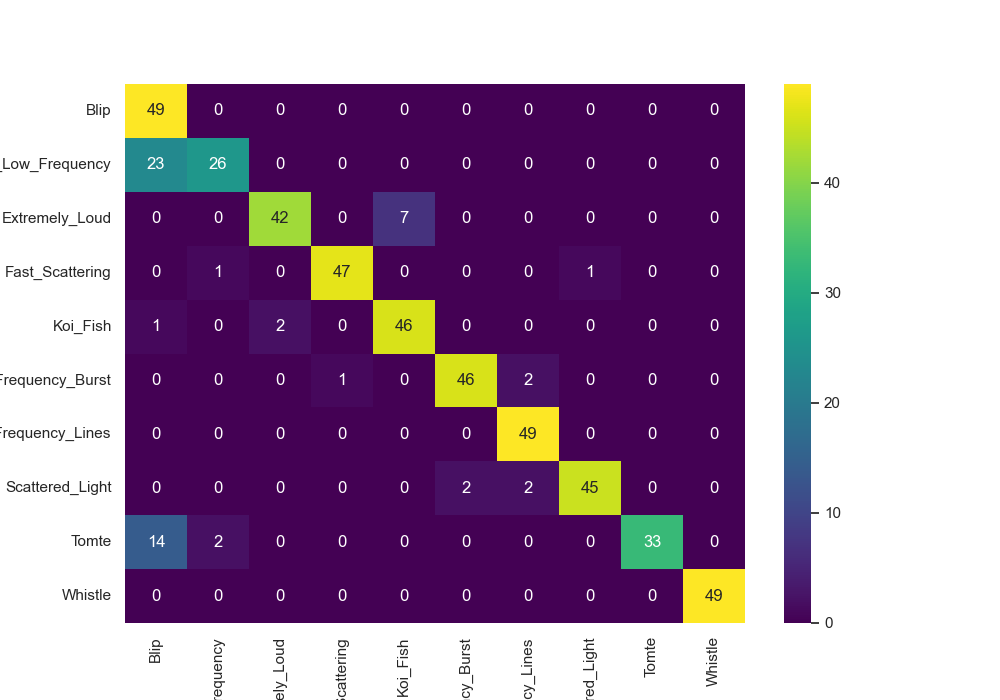
\includegraphics[width=0.49\textwidth]{Images/cm_LwF_MultiView_100epochs.png}  
  \label{fig:sub-first2}
\end{subfigure}
\begin{subfigure}
  \centering
  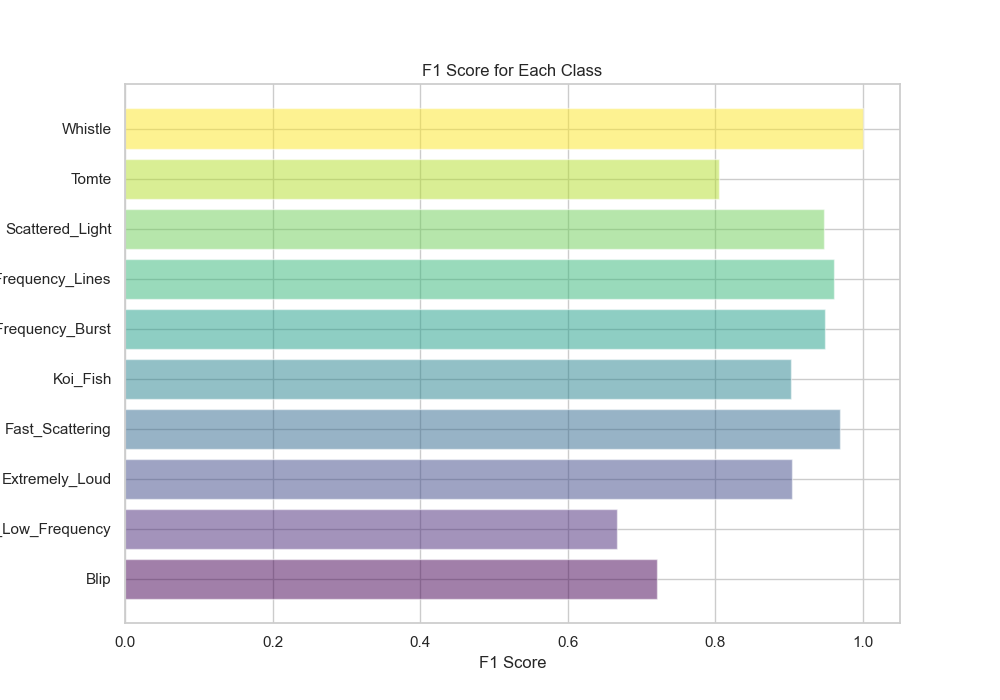
\includegraphics[width=0.49\textwidth]{Images/f1_LwF_MultiView_100epochs.png}  
  \label{fig:sub-second2}
\end{subfigure}
\caption{Confusion matrix and f1 plot for LwF strategy}
\label{fig:cm_f1_lwf_baseline}
\end{figure}

\begin{table}
\centering
    \begin{tabular}{|l|c c c|}
    \hline
    \textbf{Glitch type} & \textbf{Precision} & \textbf{Recall} & \textbf{f1-score} \\ \hline
    Blip & $0.56$ & $1.00$ & $0.72$ \\
    Blip\_Low\_Frequency & $0.90$ & $0.53$ & $0.67$\\
    Extremely\_Loud & $0.95$ & $0.86$ &  $0.90$\\
    Fast\_Scattering & $0.98$ & $0.96$ &  $0.97$\\
    Koi\_Fish & $0.87$ & $0.94$ & $0.90$\\
    Low\_Frequency\_Burst & $0.96$ & $0.94$ & $0.95$\\
    Low\_Frequency\_Lines & $0.92$ & $1.00$ & $0.96$\\
    Scattered\_Light & $0.98$ & $0.92$ &$0.95$ \\
    Tomte & $1.00$ & $0.67$ &$0.80$ \\
    Whistle & $1.00$ & $1.00$ & $1.00$ \\
    \hline
    \end{tabular}
    \caption{Classification report of the LwF strategy.}
    \label{tbl:RQ1_class_report_LWF}
\end{table}


Due to these findings, further exploration of the embedding using \acrshort{tsne} and \acrshort{umap} plots (in two dimensions) is necessary.\\ The \acrshort{tsne} and \acrshort{umap} representation, as shown in Figure \ref{fig:tSNE_LwF}, shows a clustering of glitch categories in 2D space.


\begin{figure}[ht]
\centering
    \centering
    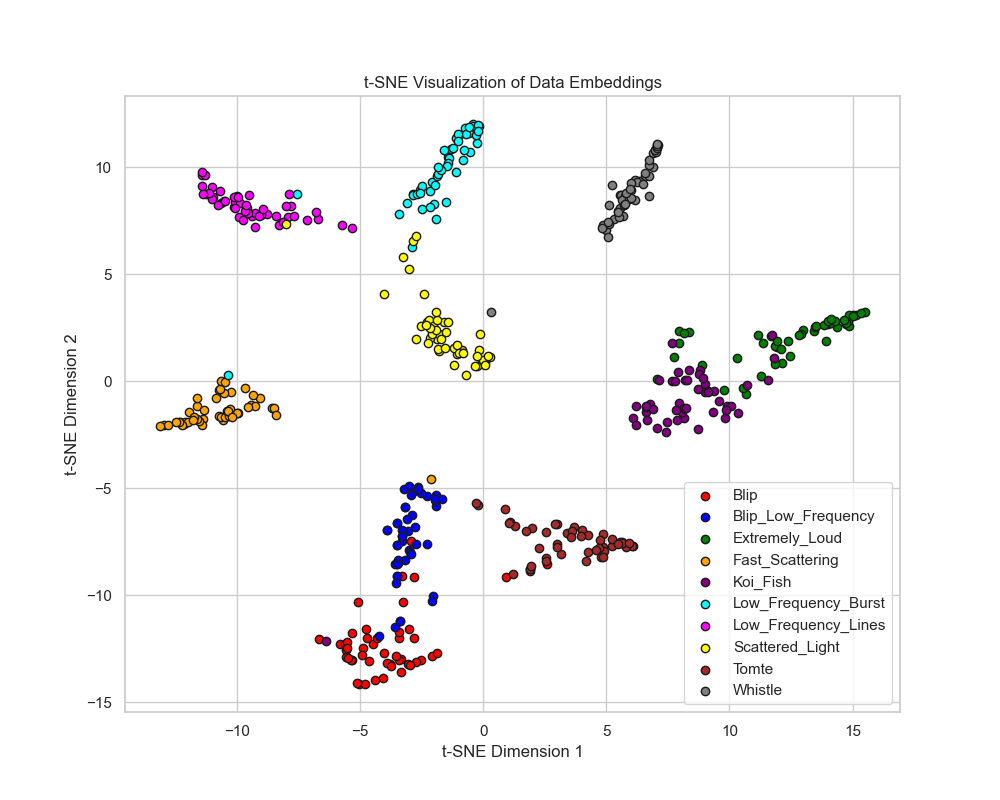
\includegraphics[width=0.6\textwidth]{Images/tSNE_LwF_MultiView_testset_100epochs.png}
    \caption{t-SNE visualization LwF}
    \label{fig:tSNE_LwF}
\end{figure}

\begin{figure}[ht]
  \centering
    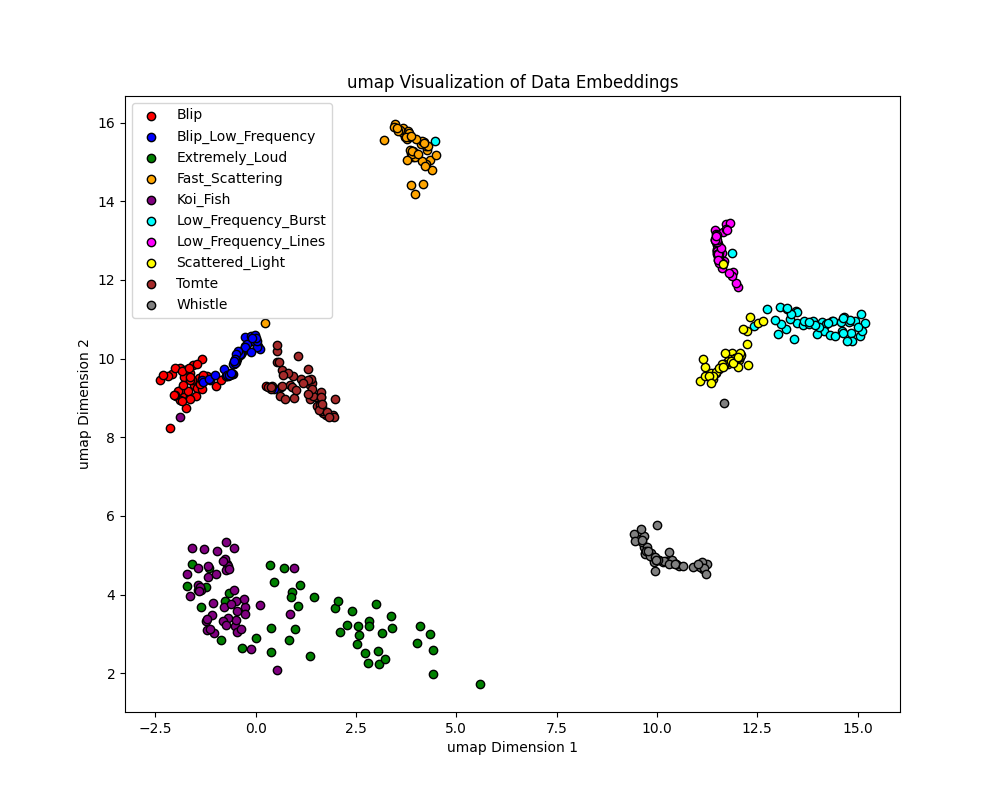
\includegraphics[width=0.6\textwidth]{Images/umap_MultiView_LwF_testset_100epochs.png}
    \caption{UMAP visualization LwF}
    \label{fig:umap_LwF}
\end{figure}


Some relevant observations that can be made: 
\begin{itemize}
    \item There seems to be a rough separation between glitches along t-SNE dimension 1. This is visible in both the t-SNE and UMAP visualization.  
    \item Potential similarities among certain glitch classes like "Koi\_Fish" and "Tomte" appear close together in the plot. This indicates that these classes share some underlying features. 
\end{itemize}

The images of the Saliency Mapping in Figure \ref{fig:saliency_lwf} show that the model attends to different regions of the spectrogram to classify different glitch types. The model makes a mistake in the top left image. This is predicted to be a 'Blip', but actually this is a 'Tomte'. 
When investigating the 'Koi\_Fish' pattern next to the 'Blip' and 'Tomte', we see that similar features are retrieved. This confirms the observations made by the t-SNE and UMAP visualizations. 

\begin{figure}[ht]
    \centering
    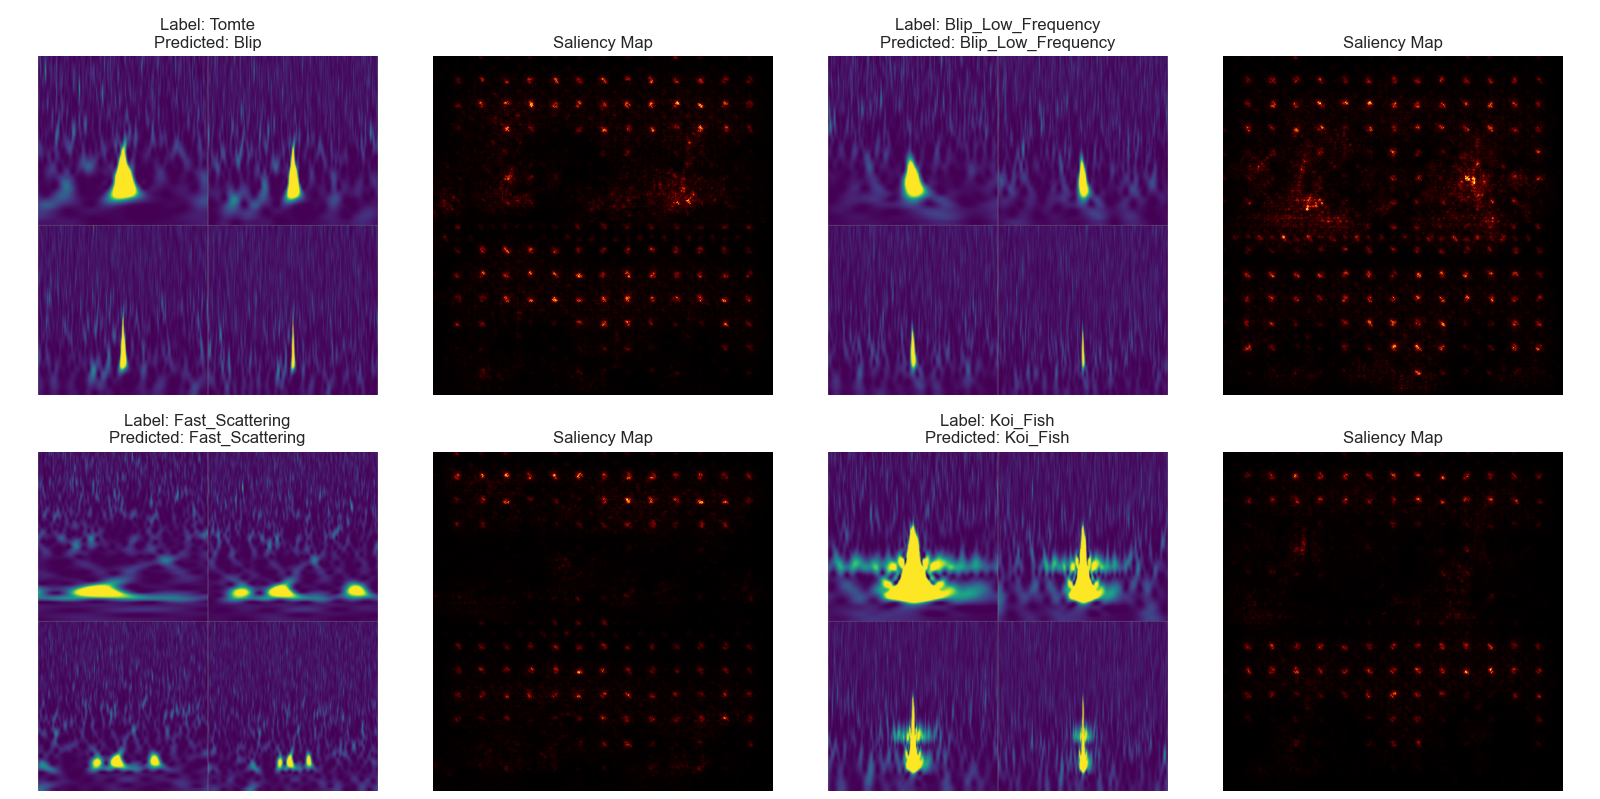
\includegraphics[width=0.95\textwidth]{Images/SaliencyMapping_LwF_MultiView_100epochs_selection.png}
    \caption{Saliency Mapping of LwF}
    \label{fig:saliency_lwf}
\end{figure}

\newpage

\subsubsection{AGEM strategy}
\label{subsubsec:RQ1_AGEM}
A second \acrshort{cl} strategy addressing catastrophic forgetting is called \acrfull{agem}. \acrshort{agem} utilises an episodic memory of gradients computed on past tasks. During training, it computes the gradient of the current model with respect to the new task's loss. It then compares the gradient with the average gradient computed on the past tasks. If the new gradient deviates significantly from the average, \acrshort{agem} adjusts the update direction to prevent catastrophic forgetting. The model is trained, just as in the naive baseline, on five distinct tasks that contain two classes per experience. 

The strategy is augmented with the \verb|ReplayPlugin| used in the previous strategy, but also an \verb|AGEMPlugin|. The \verb|AGEMPlugin| is specifically designed for \acrshort{agem} it maintains a set of past examples. 

The hyperparameter choices are: 
\begin{itemize}
    \item \verb|patterns_per_exp|: The number of patterns (samples) stored for each past experience. Based on the papers by \citep{chaudhry2018efficient, lopez2017gradient} and the fact there are 10 patterns in the benchmark, here we opt for a value of '10'. 
    \item \verb|sample_size|: The number of patterns sampled from the memory buffer during training. Here we opt for the default same sample size equal to the dataloader batch size. 
\end{itemize}


Changes in weight distribution are tracked for illustrative purposes and shown in Figure \ref{fig:agem_weight_distribution}

\begin{figure}[ht]
\centering
\begin{subfigure}
  \centering
  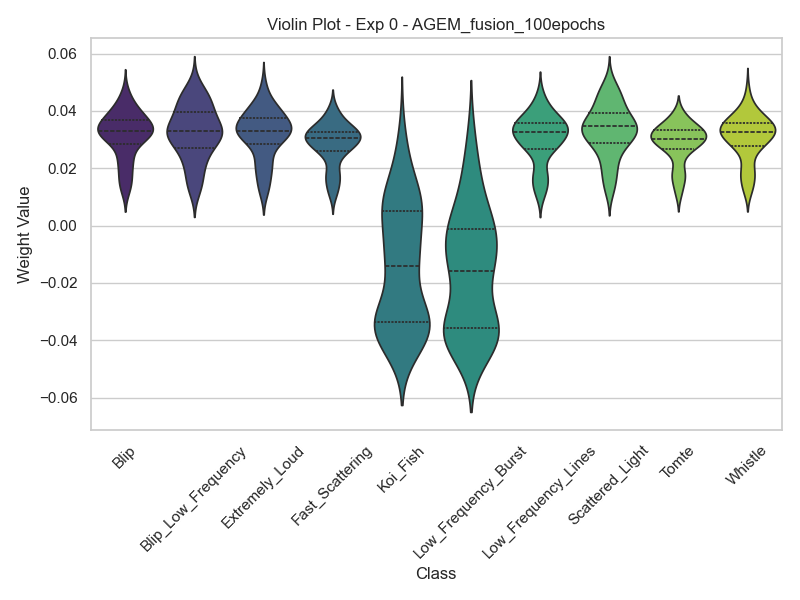
\includegraphics[width=0.4\textwidth]{Grad Assignment/Images/AGEM_fusion_100epochs_exp_0.png}  
  \label{fig:agem_violin_exp_0}
\end{subfigure}
\begin{subfigure}
  \centering
  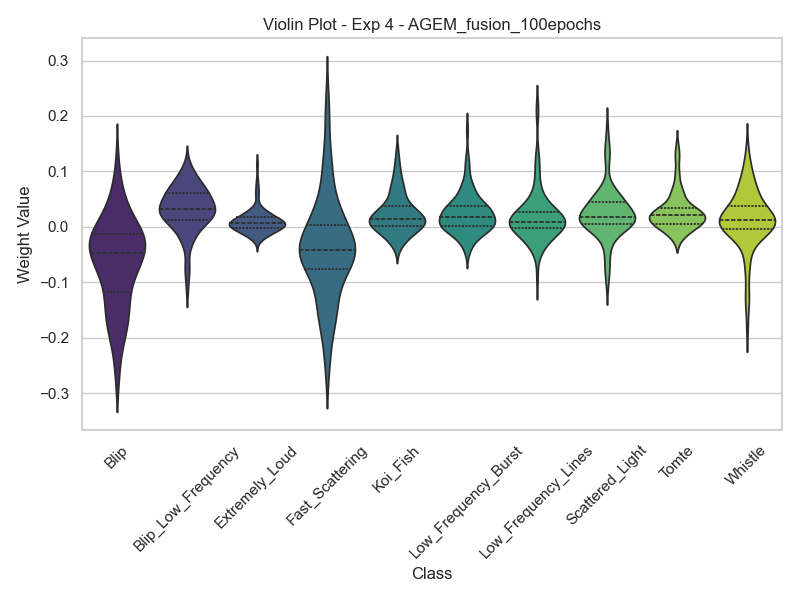
\includegraphics[width=0.4\textwidth]{Grad Assignment/Images/AGEM_fusion_100epochs_exp_4.png}  
  \label{fig:agem_violin_exp_4}
\end{subfigure}
\caption{Weight distribution changes}
\label{fig:agem_weight_distribution}
\end{figure}

From the Confusion Matrix, f1 plot and Classification report as shown in Figure \ref{fig:cm_f1_agem_baseline} and Table \ref{tbl:RQ1_class_report_agem} we find that the overall accuracy is $87 \%$, one percent point lower than the LwF results as depicted in \ref{subsubsec:RQ1_LWF}. The model performs well on the majority of classes, but struggles with 'Tomte' and 'Blip\_Low\_Frequency'. Especially the recall on 'Tomte' is very low, indicating a high number of False Negatives. On the other hand, if the 'Tomte' glitch class is detected, the model is very reliable (high precision). 

\begin{figure}[H]
\centering
\begin{subfigure}
  \centering
  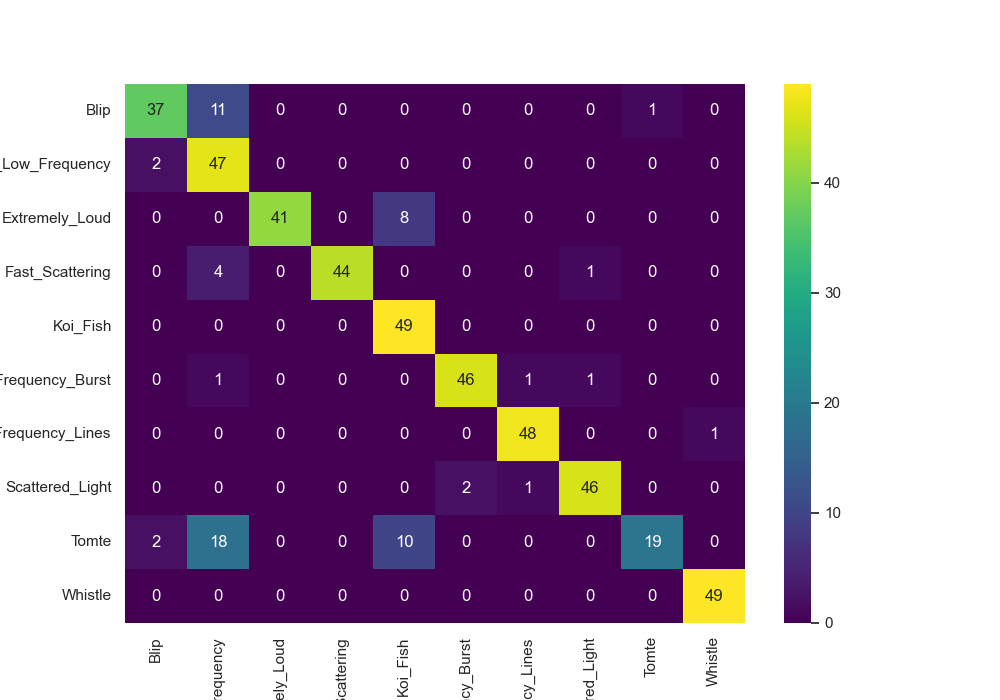
\includegraphics[width=0.49\textwidth]{Images/cm_AGEM_MultiView_100epochs.png}  
  \label{fig:sub-first3}
\end{subfigure}
\begin{subfigure}
  \centering
  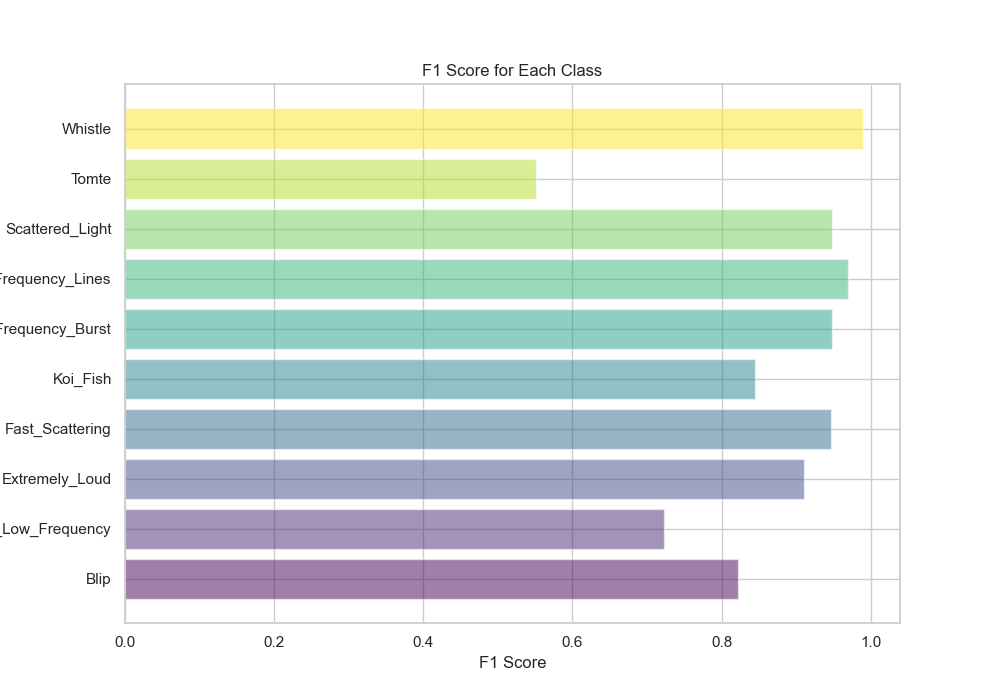
\includegraphics[width=0.49\textwidth]{Grad Assignment/Images/f1_AGEM_MultiView_100epochs.png}  
  \label{fig:sub-second3}
\end{subfigure}
\caption{Confusion matrix and f1 plot for AGEM strategy}
\label{fig:cm_f1_agem_baseline}
\end{figure}

\begin{table}
\centering

    \begin{tabular}{|l|c c c|}
    \hline
    \textbf{Glitch type} & \textbf{Precision} & \textbf{Recall} & \textbf{f1-score} \\ \hline
    Blip & $0.90$ & $0.76$ & $0.82$ \\
    Blip\_Low\_Frequency & $0.58$ & $0.96$ & $0.72$\\
    Extremely\_Loud & $0.1.00$ & $0.84$ &  $0.91$\\
    Fast\_Scattering & $1.00$ & $0.90$ &  $0.95$\\
    Koi\_Fish & $0.73$ & $1.00$ & $0.84$\\
    Low\_Frequency\_Burst & $0.96$ & $0.94$ & $0.95$\\
    Low\_Frequency\_Lines & $0.96$ & $0.98$ & $0.97$\\
    Scattered\_Light & $0.96$ & $0.94$ &$0.95$ \\
    Tomte & $0.95$ & $0.39$ &$0.55$ \\
    Whistle & $0.98$ & $1.00$ & $0.99$ \\
    \hline
    \end{tabular}
    \caption{Classification report of the AGEM strategy.}
    \label{tbl:RQ1_class_report_agem}
\end{table}

Similar findings can be found from the investigation of the embedding space using \acrshort{tsne} and \acrshort{umap} plots in Figure \ref{fig:tsne_umap_AGEM},.

\begin{figure}[ht]
\centering
\begin{subfigure}
    \centering
    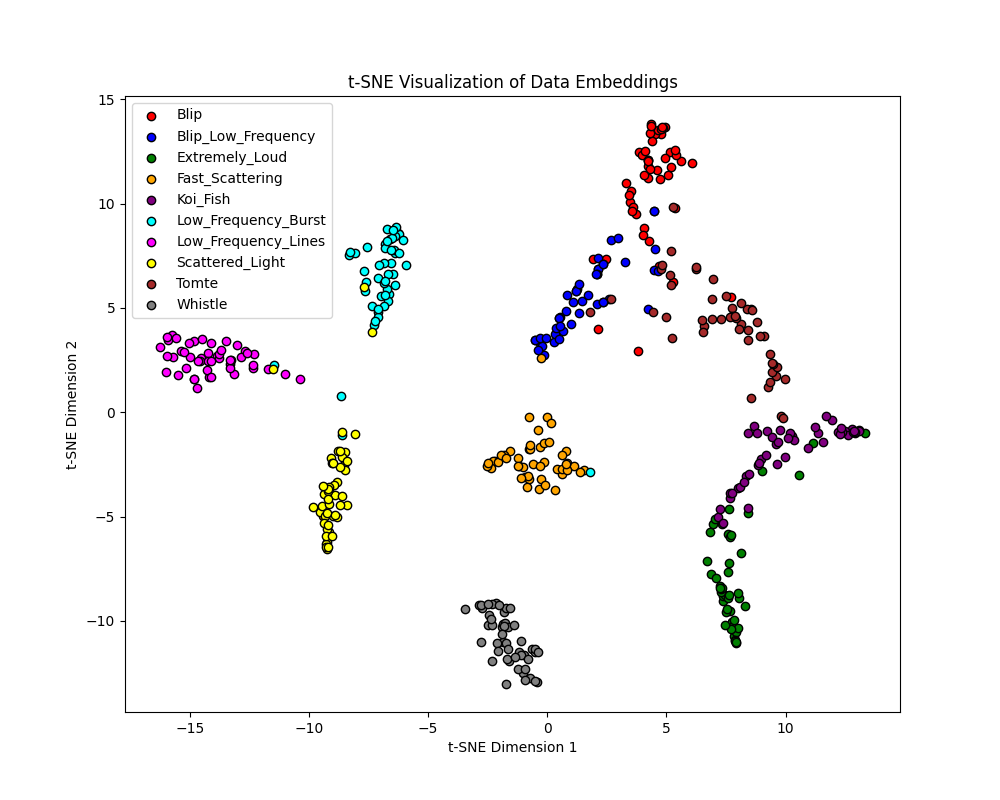
\includegraphics[width=0.45\textwidth]{Images/tSNE_AGEM_MultiView_testset_100epochs.png}
\end{subfigure}
\begin{subfigure}
    \centering
    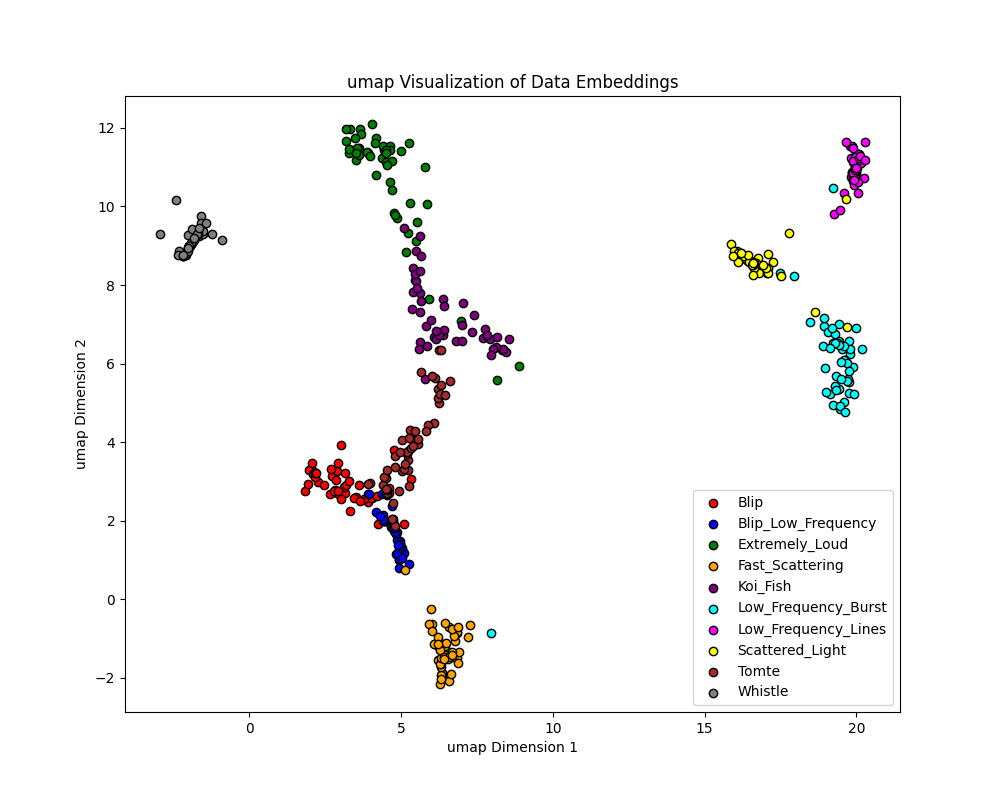
\includegraphics[width=0.45\textwidth]{Images/umap_MultiView_AGEM_testset_100epochs.png}
\end{subfigure}
    \caption{t-SNE and UMAP visualisation of the AGEM strategy.}
    \label{fig:tsne_umap_AGEM}
\end{figure}
Example saliency mappings can be found in Appendix \ref{appendix4}.  
\newpage

\subsubsection{EWC strategy}
\label{subsubsec:RQ1_EWC}
A third \acrshort{cl} strategy addressing catastrophic forgetting is called \acrfull{ewc}. \acrshort{ewc} acts like a memory preserver in neural networks. During training on new experiences, \acrshort{ewc} penalizes large updates to important weights used in previous tasks. This gentles the learning process, allowing the network to adapt to new information while retaining previously learned knowledge, hence avoiding recency bias. \\


The strategy is augmented with the \verb|ReplayPlugin| used in the previous strategies. An extra hyperparameter, \verb|ewc_lambda|, must be selected. We choose a value of $\lambda = 0.1$, signifying a moderate penalty for weight updates when training on new tasks. Typically, a greater value (approaching 1) emphasizes the preservation of previous knowledge, although it may hinder the acquisition of new skills.

\begin{figure}[H]
\centering
\begin{subfigure}
  \centering
  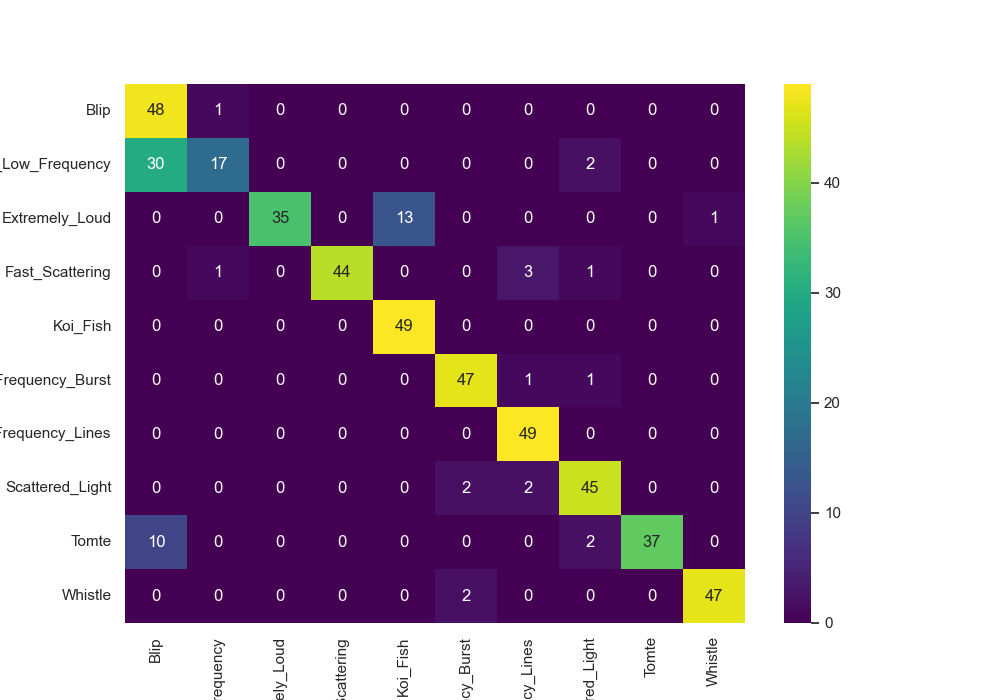
\includegraphics[width=0.49\textwidth]{Images/cm_EWC_MultiView_100epochs.png}  
  \label{fig:sub-first4}
\end{subfigure}
\begin{subfigure}
  \centering
  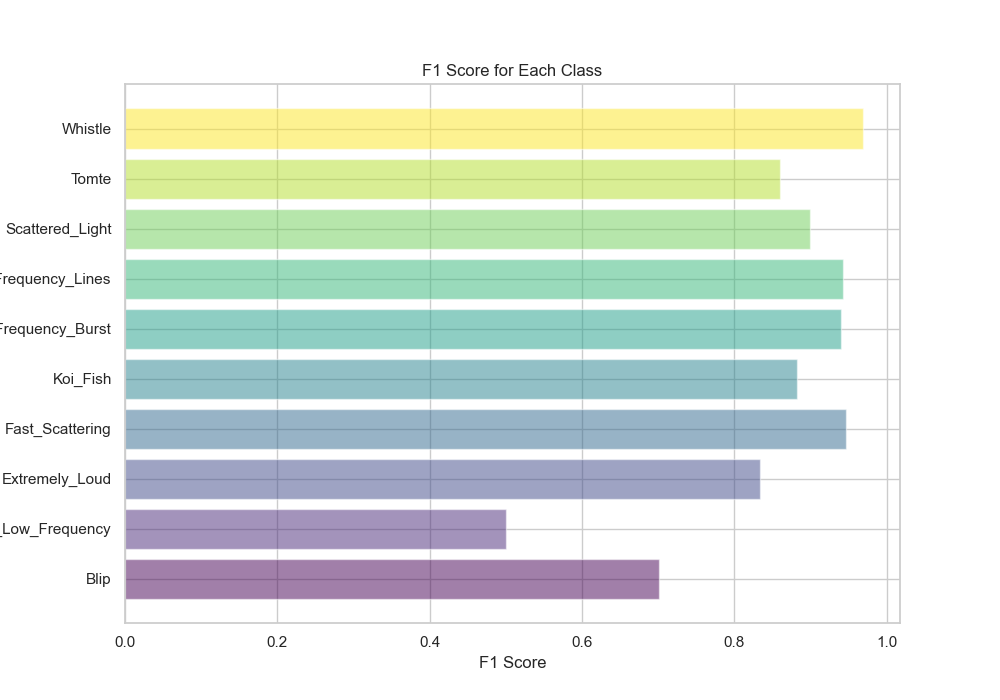
\includegraphics[width=0.49\textwidth]{Images/f1_EWC_MultiView_100epochs.png}  
  \label{fig:sub-second4}
\end{subfigure}
\caption{Confusion matrix and f1 plot for EWC strategy}
\label{fig:cm_f1_ewc_baseline}
\end{figure}

\begin{table}[ht]
\centering
    \begin{tabular}{|l|c c c|}
    \hline
    \textbf{Glitch type} & \textbf{Precision} & \textbf{Recall} & \textbf{f1-score} \\ \hline
    Blip & $0.55$ & $0.98$ & $0.70$ \\
    Blip\_Low\_Frequency & $0.89$ & $0.35$ & $0.50$\\
    Extremely\_Loud & $1.00$ & $0.71$ &  $0.83$\\
    Fast\_Scattering & $1.00$ & $0.90$ &  $0.95$\\
    Koi\_Fish & $0.79$ & $1.00$ & $0.88$\\
    Low\_Frequency\_Burst & $0.92$ & $0.96$ & $0.94$\\
    Low\_Frequency\_Lines & $0.89$ & $1.00$ & $0.94$\\
    Scattered\_Light & $0.88$ & $0.92$ &$0.90$ \\
    Tomte & $1.00$ & $0.76$ & $0.86$ \\
    Whistle & $0.98$ & $0.96$ & $0.97$ \\
    \hline
    \end{tabular}
    \caption{Classification report of the EWC strategy.}
    \label{tbl:RQ1_class_report_ewc}
\end{table}


From the Confusion Matrix, f1 plot and Classification report as shown in Figure \ref{fig:cm_f1_ewc_baseline} and Table \ref{tbl:RQ1_class_report_ewc} we find that the overall accuracy is $85 \%$, several percent points lower than the previous best LwF results as depicted in \ref{subsubsec:RQ1_LWF}. The model performs well on the majority of classes, but struggles with 'Blip' and 'Blip\_Low\_Frequency'. Especially the recall on 'Blip\_Low\_Frequency' is very low.

\newpage
\subsubsection{DER strategy}
\label{subsubsec:RQ1_DER}
\acrfull{der} combats recency bias by replaying past predictions, acting like a teacher. It stores the model's past outputs (logits) from old tasks alongside the original data. During training on new experiences (new classes), \acrshort{der} forces the model's current predictions on old data to align with its past predictions, reminding it of what it already knew, thus hindering catastrophic forgetting. \\
The hyperparameter \verb|alpha| controls the weight given to the replay loss (from past predictions) compared to the current task loss. A value of $\alpha = 1.0$ means that the replay loss is given equal importance to the current task loss during training on new experiences. Basically the model must optimize two things equally: 1) Fitting the new data and 2) Staying consistent with past predictions \citep{buzzega2020dark}.
\begin{figure}[H]
\centering
\begin{subfigure}
  \centering
  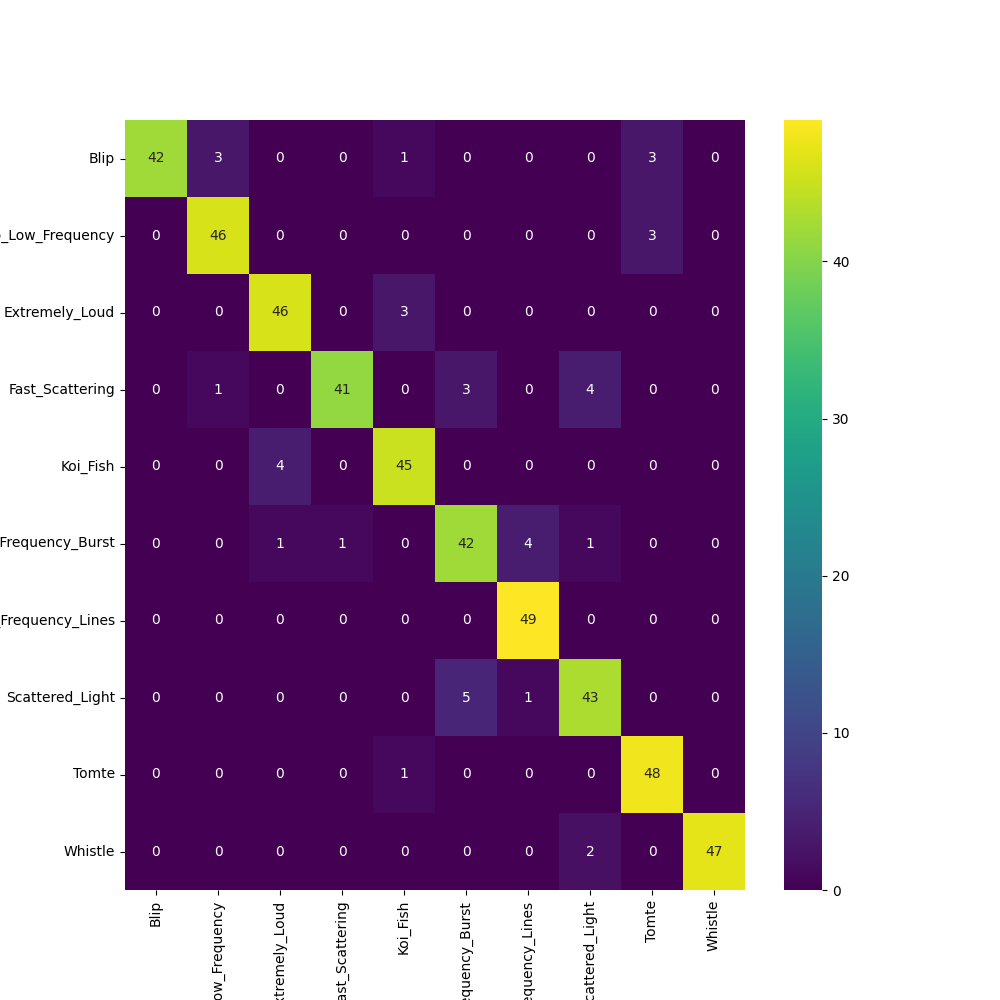
\includegraphics[width=0.49\textwidth]{Images/cm_DER_MultiView_100epochs.png}  
  \label{fig:sub-first5}
\end{subfigure}
\begin{subfigure}
  \centering
  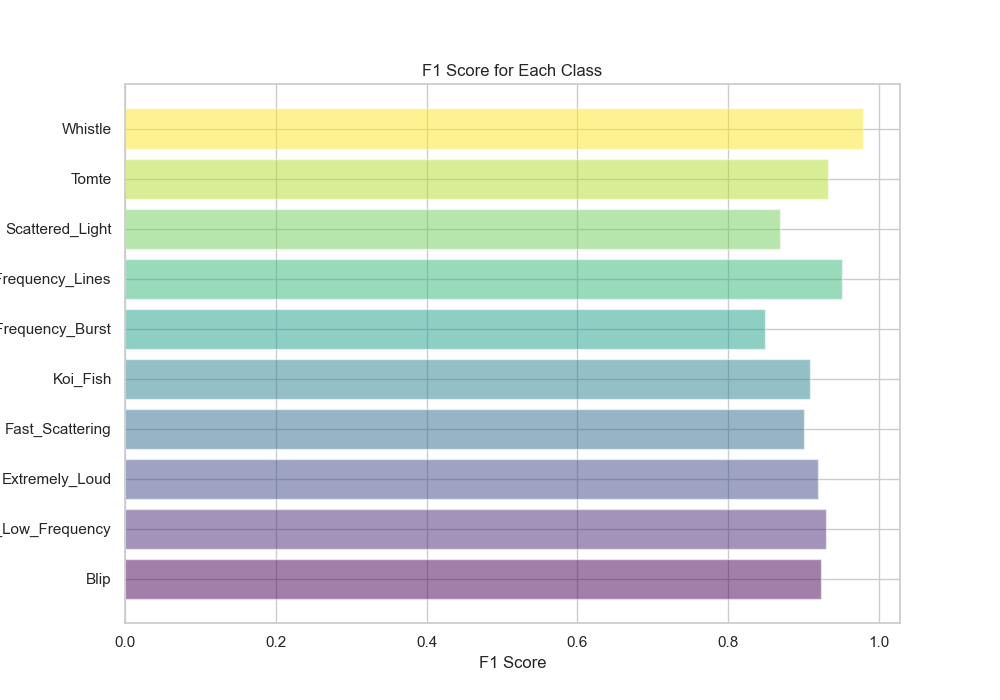
\includegraphics[width=0.49\textwidth]{Images/f1_DER_MultiView_100epochs.png}  
  \label{fig:sub-second5}
\end{subfigure}
\caption{Confusion matrix and f1 plot for DER strategy}
\label{fig:cm_f1_der_baseline}
\end{figure}
\begin{table}[ht]
\centering
    \begin{tabular}{|l|c c c|}
    \hline
    \textbf{Glitch type} & \textbf{Precision} & \textbf{Recall} & \textbf{f1-score} \\ \hline
    Blip & $1.00$ & $0.86$ & $0.92$ \\
    Blip\_Low\_Frequency & $0.92$ & $0.94$ & $0.93$\\
    Extremely\_Loud & $0.90$ & $0.94$ &  $0.92$\\
    Fast\_Scattering & $0.98$ & $0.84$ &  $0.90$\\
    Koi\_Fish & $0.90$ & $0.92$ & $0.91$\\
    Low\_Frequency\_Burst & $0.84$ & $0.86$ & $0.85$\\
    Low\_Frequency\_Lines & $0.91$ & $1.00$ & $0.95$\\
    Scattered\_Light & $0.86$ & $0.88$ &$0.87$ \\
    Tomte & $0.89$ & $0.98$ & $0.93$ \\
    Whistle & $1.00$ & $0.96$ & $0.98$ \\
    \hline
    \end{tabular}
    \caption{Classification report of the DER strategy.}
    \label{tbl:RQ1_class_report_der}
\end{table}

From the Confusion Matrix, f1 plot and Classification report as shown in Figure \ref{fig:cm_f1_der_baseline} and Table \ref{tbl:RQ1_class_report_der} we find that the overall accuracy is $92\%$, more than the previous best \acrshort{lwf} strategy from \ref{subsubsec:RQ1_LWF}.\\

Because of the good results, it is noteworthy to further investigate the \acrshort{tsne} and \acrshort{umap} visualisations in Figure \ref{fig:tsne_umap_der}. 


\begin{figure}[ht]
\centering
\begin{subfigure}
    \centering
    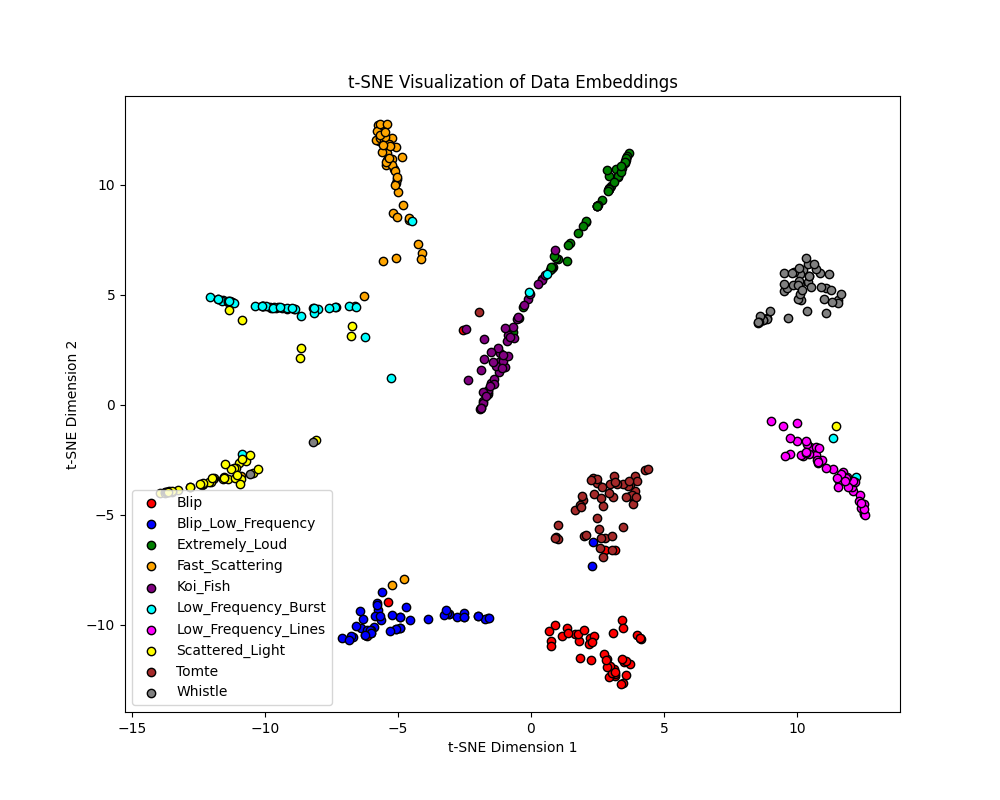
\includegraphics[width=0.45\textwidth]{Images/tSNE_DER_MultiView_testset_100epochs.png}
\end{subfigure}
\begin{subfigure}
    \centering
    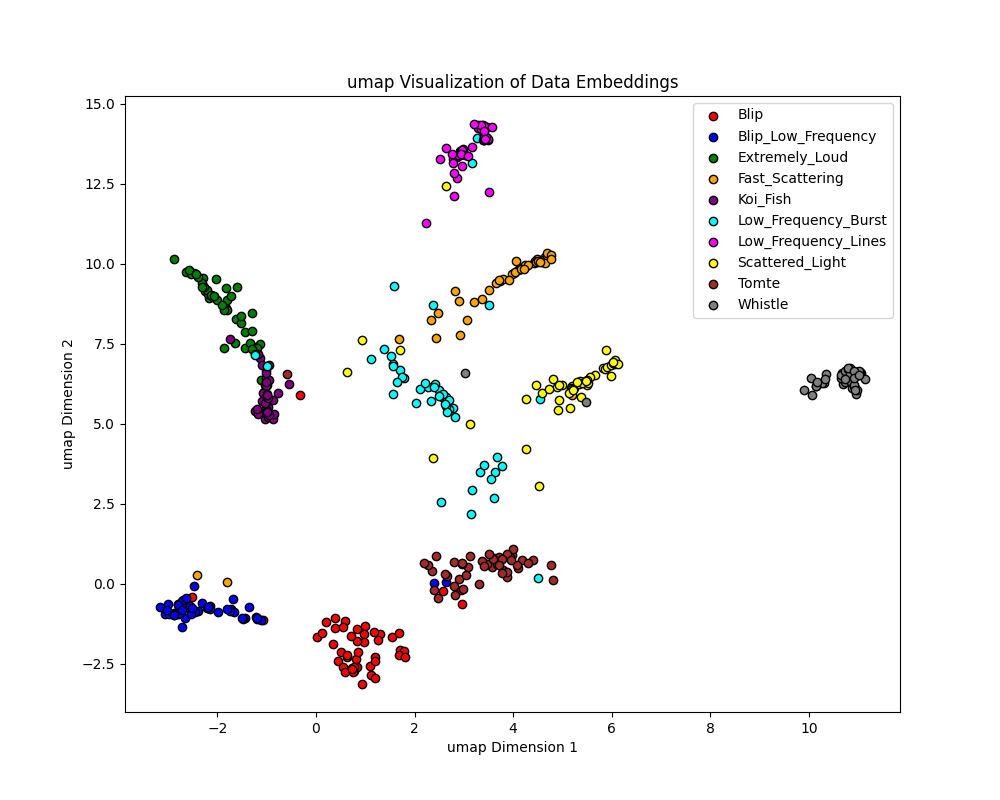
\includegraphics[width=0.45\textwidth]{Images/umap_MultiView_DER_testset_100epochs.png}
\end{subfigure}
    \caption{t-SNE and UMAP visualisation of the DER strategy.}
    \label{fig:tsne_umap_der}
\end{figure}

Some relevant observations that can be made: 
\begin{itemize}
    \item The separation between 'Blip', 'Blip\_Low\_Frequency' and 'Tomte' is more defined as opposed to the previous best results. 
    \item \acrshort{der} seems to have more troubles with distinguishing 'Extremely\_Loud' and 'Koi\_Fish' glitch types. 
\end{itemize}

The images of the Saliency Mapping in Figure \ref{fig:saliency_der} visualise the above made observations more clearly. 

\begin{figure}[ht]
    \centering
    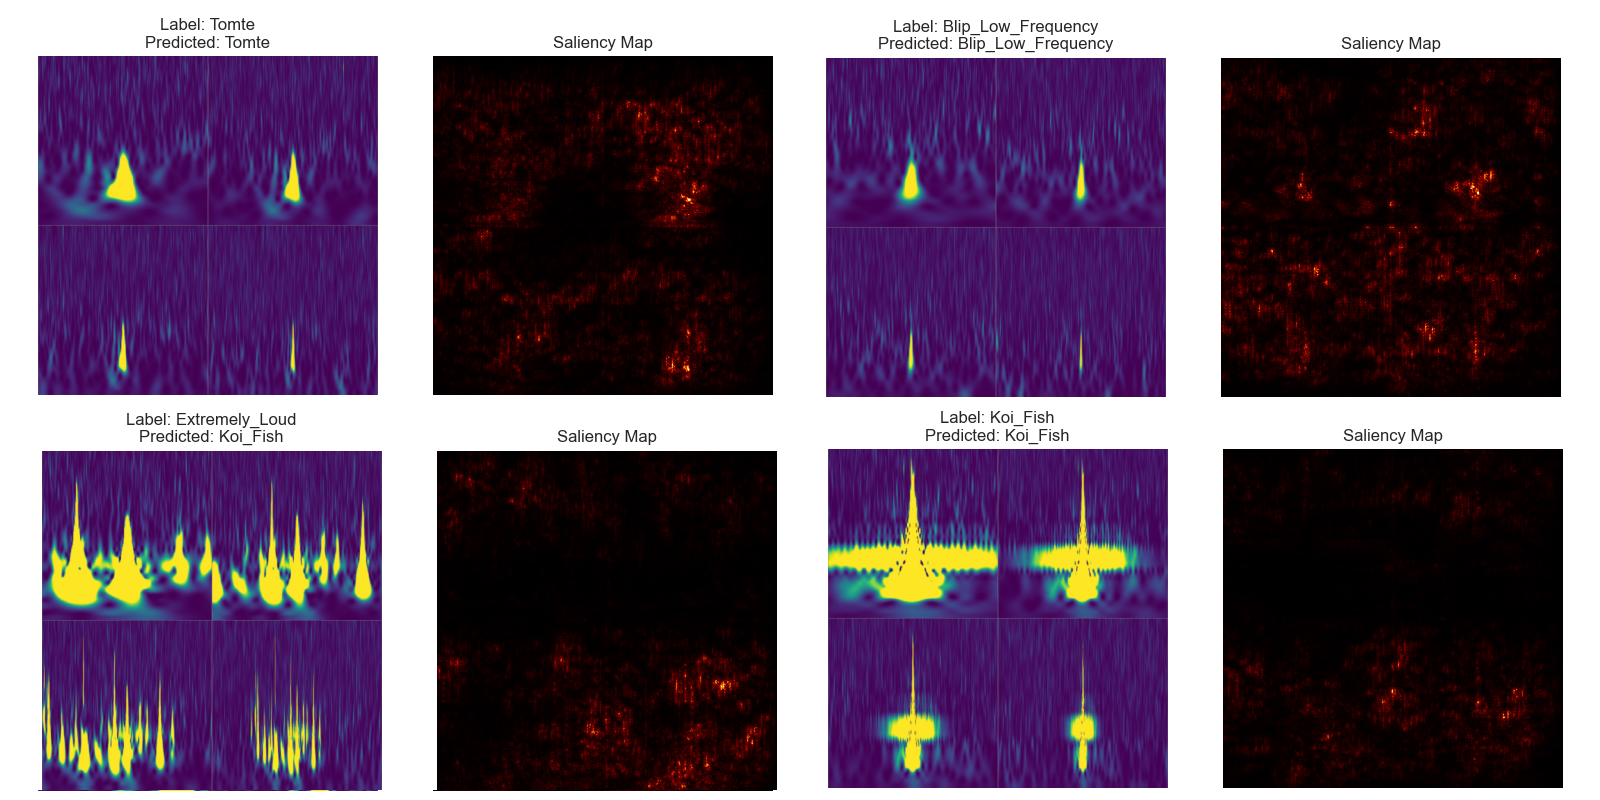
\includegraphics[width=0.95\textwidth]{Grad Assignment/Images/SaliencyMapping_DER_MultiView_100epochs_selection.png}
    \caption{Saliency Mapping of DER}
    \label{fig:saliency_der}
\end{figure}
\newpage

\subsubsection{DER++ strategy}
\label{subsubsec:RQ1_DER++}
\acrfull{der++} is an advanced version of \acrshort{der} from \ref{subsubsec:RQ1_DER}. It extends the replay buffer by also storing the ground truth logits and replay examples \citep{buzzega2020dark}. \acrshort{der++} mitigates, in this way, the shortcoming of \acrshort{der} that weakens when the logits are highly biased due to a sudden distribution shift \citep{ling2022difficulty}. 

\begin{figure}[H]
\centering
\begin{subfigure}
  \centering
  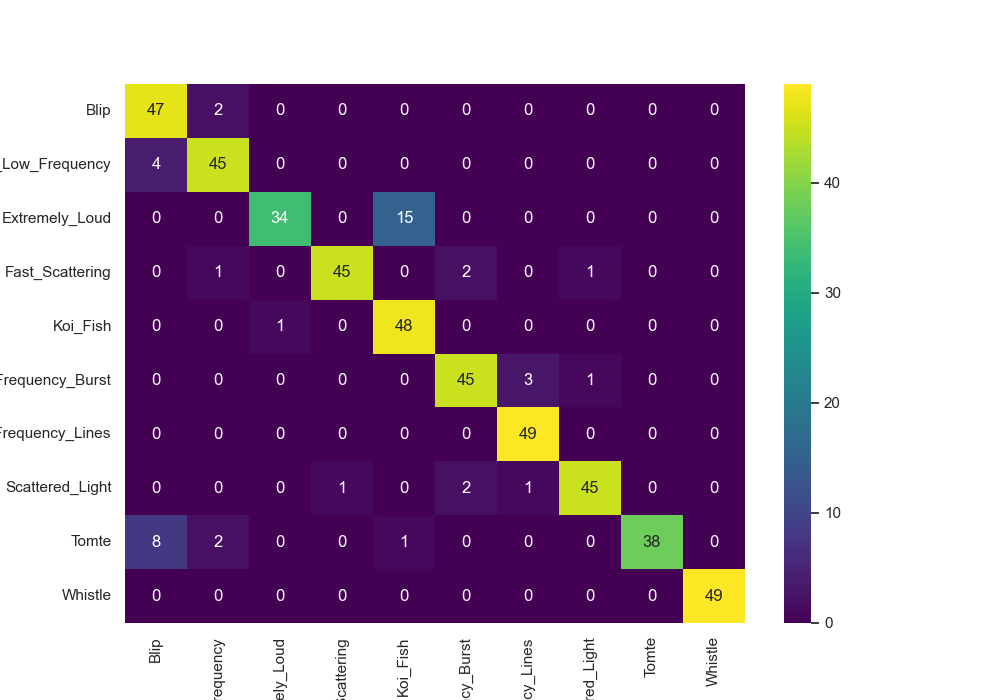
\includegraphics[width=0.49\textwidth]{Images/cm_DER++_MultiView_100epochs.png}  
  \label{fig:sub-first6}
\end{subfigure}
\begin{subfigure}
  \centering
  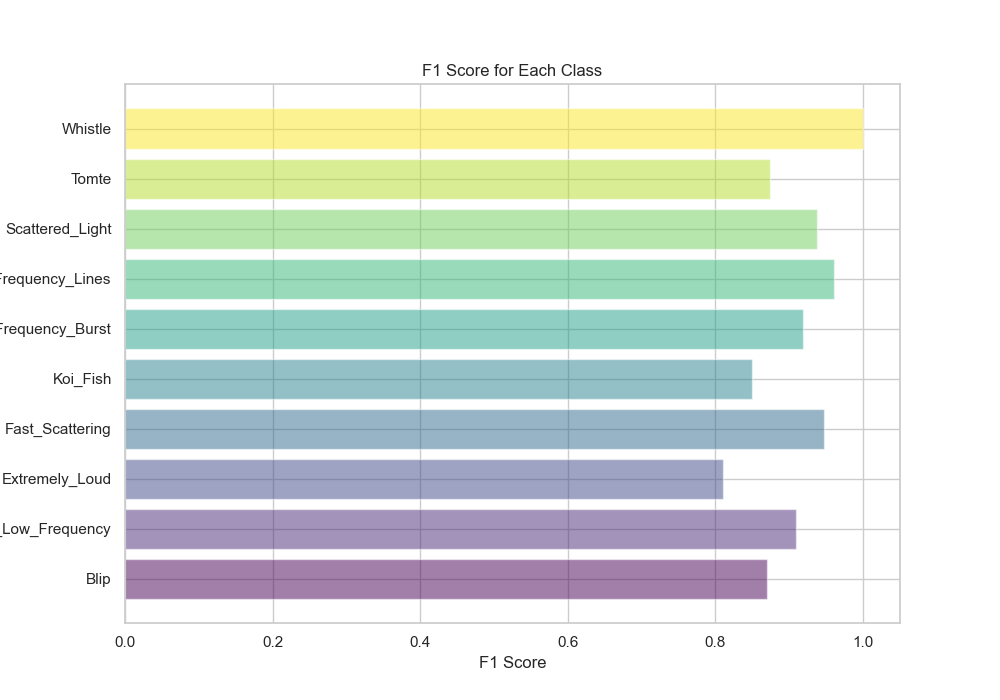
\includegraphics[width=0.49\textwidth]{Images/f1_DER++_MultiView_100epochs.png}  
  \label{fig:sub-second6}
\end{subfigure}
\caption{Confusion matrix and f1 plot for DER++ strategy}
\label{fig:cm_f1_der++_baseline}
\end{figure}
\begin{table}[ht]
\centering
    \begin{tabular}{|l|c c c|}
    \hline
    \textbf{Glitch type} & \textbf{Precision} & \textbf{Recall} & \textbf{f1-score} \\ \hline
    Blip & $0.80$ & $0.96$ & $0.87$ \\
    Blip\_Low\_Frequency & $0.90$ & $0.92$ & $0.91$\\
    Extremely\_Loud & $0.97$ & $0.69$ &  $0.81$\\
    Fast\_Scattering & $0.98$ & $0.92$ &  $0.95$\\
    Koi\_Fish & $0.75$ & $0.98$ & $0.85$\\
    Low\_Frequency\_Burst & $0.92$ & $0.92$ & $0.92$\\
    Low\_Frequency\_Lines & $0.92$ & $1.00$ & $0.96$\\
    Scattered\_Light & $0.96$ & $0.92$ & $0.94$ \\
    Tomte & $1.00$ & $0.78$ & $0.87$ \\
    Whistle & $1.00$ & $1.00$ & $1.00$ \\
    \hline
    \end{tabular}
    \caption{Classification report of the DER++ strategy.}
    \label{tbl:RQ1_class_report_der++}
\end{table}

From the Confusion Matrix, f1 plot and Classification report as shown in Figure \ref{fig:cm_f1_der++_baseline} and Table \ref{tbl:RQ1_class_report_der++} we find that the overall accuracy is $91\%$, one percent point less than the previous best \acrshort{der} strategy from \ref{subsubsec:RQ1_DER}. It has perfect results on 'Whistle' and 'Low\_Frequency\_Lines' glitches. \\

\newpage
\subsubsection{SCR strategy}
\label{subsub:RQ1_SCR}
As described in \ref{sec:SCR}, \acrshort{scr} leverages the Nearest-Class-Mean classifier as a substitute for the Softmax classifier by addressing recency bias and avoiding structural changes in the fully-connected layer for new classes. There is however a risk involved, the effectiveness of \acrshort{scr} might depend on the quality of the data embeddings and the between-class separation. It also has the tendency of introducing additional bias \citep{mai2021supervised, aleixo2023catastrophic}.   

\begin{figure}[H]
\centering
\begin{subfigure}
  \centering
  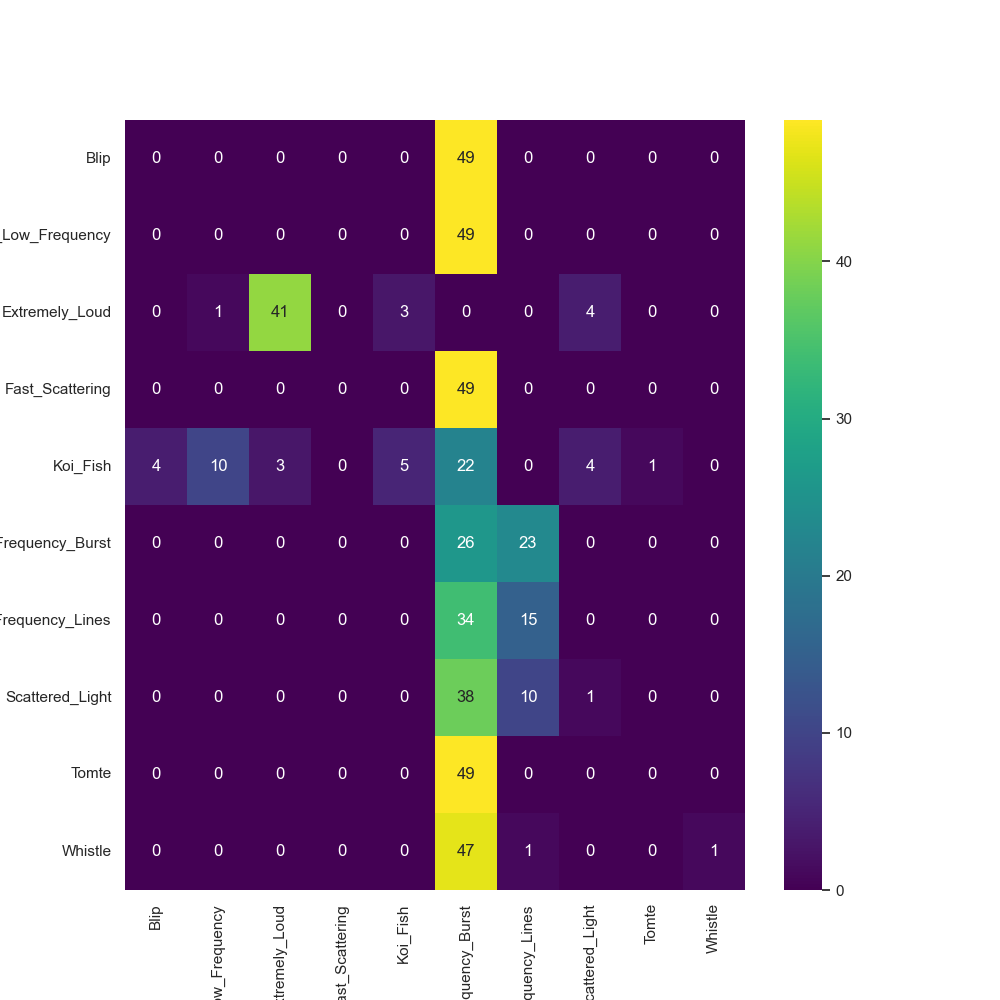
\includegraphics[width=0.49\textwidth]{Images/cm_SCR_MultiView_50epochs.png}  
  \label{fig:sub-first7}
\end{subfigure}
\begin{subfigure}
  \centering
  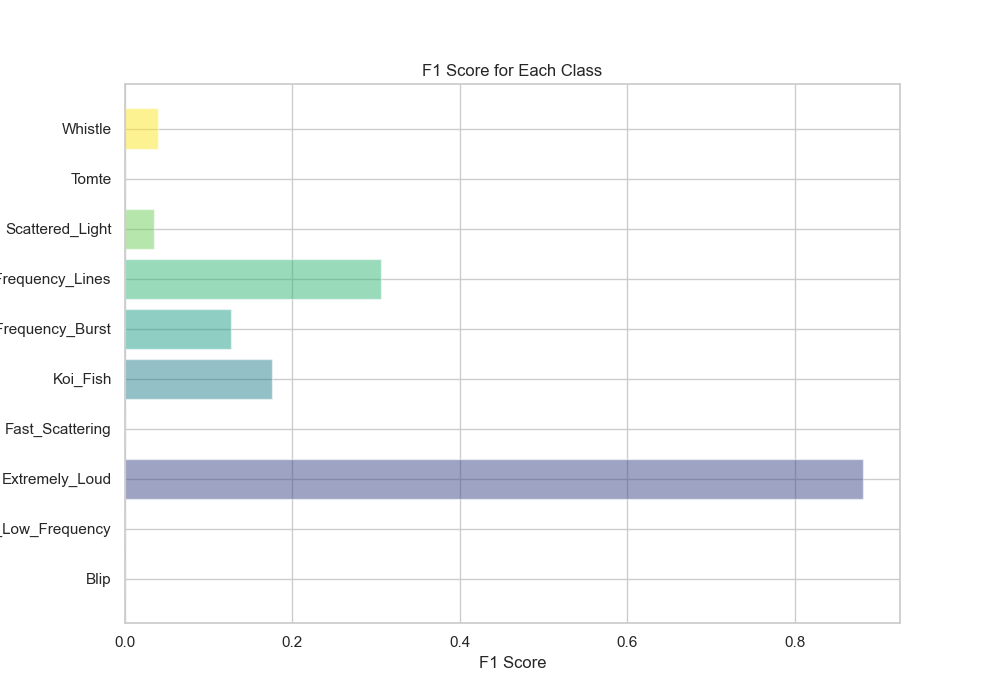
\includegraphics[width=0.49\textwidth]{Images/f1_SCR_MultiView_50epochs.png}  
  \label{fig:sub-second7}
\end{subfigure}
\caption{Confusion matrix and f1 plot for SCR strategy}
\label{fig:cm_f1_scr_baseline}
\end{figure}
\begin{table}[ht]
\centering
    \begin{tabular}{|l|c c c|}
    \hline
    \textbf{Glitch type} & \textbf{Precision} & \textbf{Recall} & \textbf{f1-score} \\ \hline
    Blip & $0.64$ & $0.80$ & $0.71$ \\
    Blip\_Low\_Frequency & $0.78$ & $0.82$ & $0.80$\\
    Extremely\_Loud & $0.96$ & $0.88$ &  $0.91$\\
    Fast\_Scattering & $0.92$ & $0.92$ &  $0.92$\\
    Koi\_Fish & $0.79$ & $0.98$ & $0.87$\\
    Low\_Frequency\_Burst & $0.96$ & $0.88$ & $0.91$\\
    Low\_Frequency\_Lines & $0.97$ & $0.78$ & $0.86$\\
    Scattered\_Light & $0.79$ & $1.00$ & $0.88$ \\
    Tomte & $0.86$ & $0.51$ & $0.64$ \\
    Whistle & $1.00$ & $0.98$ & $0.99$ \\
    \hline
    \end{tabular}
    \caption{Classification report of the SCR strategy.}
    \label{tbl:RQ1_class_report_scr}
\end{table}

From the Confusion Matrix, f1 plot and Classification report as shown in Figure \ref{fig:cm_f1_scr_baseline} and Table \ref{tbl:RQ1_class_report_scr} we find that the overall accuracy is $85\%$, worse than the best performing \acrshort{der} strategy from \ref{subsubsec:RQ1_DER}. It has good results on 'Whistle' and Fast\_Scattering' glitches. But fails greatly on 'Tomte' and 'Blip' glitches.
The training time of the implementation used in the \verb|Avalanche| package\footnote{avalanche.training.SCR at  \url{https://shorturl.at/ewOU3}} takes very long, almost three times (2.5 days) longer than \ref{subsubsec:RQ1_DER}. 

\subsection{RQ2}
\label{subsec:RQ2}
Each of the strategies are trained for 15 epochs on every task (of learning the weights on the three classes). More training epochs resulted in overfitting behavior. Between 10 and 15 epochs of training the results converge. The order in which the classes are fed is kept the same over all strategies (1 = \{Whistle\}, 2 = \{Scattered\_Light \}, 3 = \{Tomte \}).

\subsubsection{Naive CL strategy (baseline)}
\label{subsubsec:RQ2_naive}
As baseline we use the \acrshort{cl} stategy 'Naive', the hyperparameter choices and additional plugins are similar to those in \ref{subsubsec:RQ1_naive_baseline}. One difference, the benchmark consists of 3 experiences where each experience contains instances of 1 class only. 
During training we track the weight distribution changes via violin distribution plots. In the following table, \ref{tbl:naive_fd_weights}, the violin plots for the second and last experience are shown.
After the first 15 epochs training on differentiating the classes from experience 0 to 2 we get: 
\begin{center}
\begin{tabular}{cc}
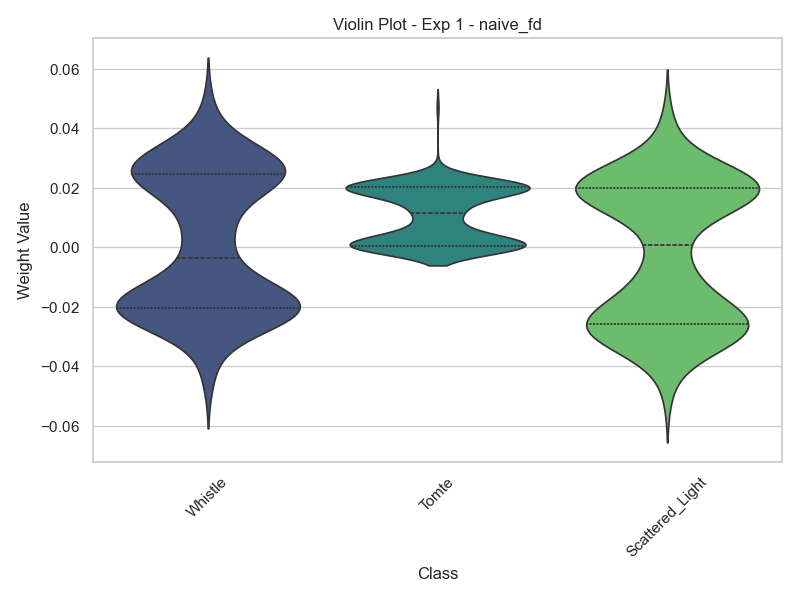
\includegraphics[width=0.4\textwidth]{Images/naive_fd_exp_1.png} & 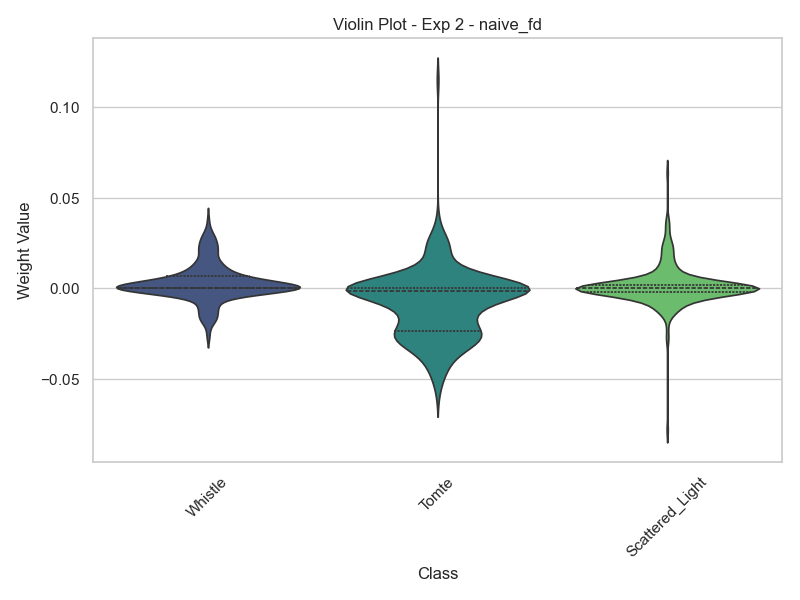
\includegraphics[width=0.4\textwidth]{Images/naive_fd_exp_2.png} \\
\end{tabular}
\label{tbl:naive_fd_weights}
\end{center}
The model has an overall accuracy of $94 \%$ and a Backward Transfer (BWT) metric of $0.0523$, indicating that the model was successful in mitigating forgetting on the old task while the model learned the new task. A similar conclusion can be made from the Confusion matrix in Figure \ref{fig:cm_f1_FD_naive_baseline} and classification report. 
The model performs well on the 'Whistle' and 'Scattered\_Light' class, but struggles some more with 'Tomte'. The F1 scores for two of the classes 'Whistle' and 'Scattered\_Light' are above 0.9, the lowest being the 'Tomte' result with F1$=0.89$, scores above 0.9 are considered very good. 

\begin{figure}[H]
\centering
\begin{subfigure}
  \centering
  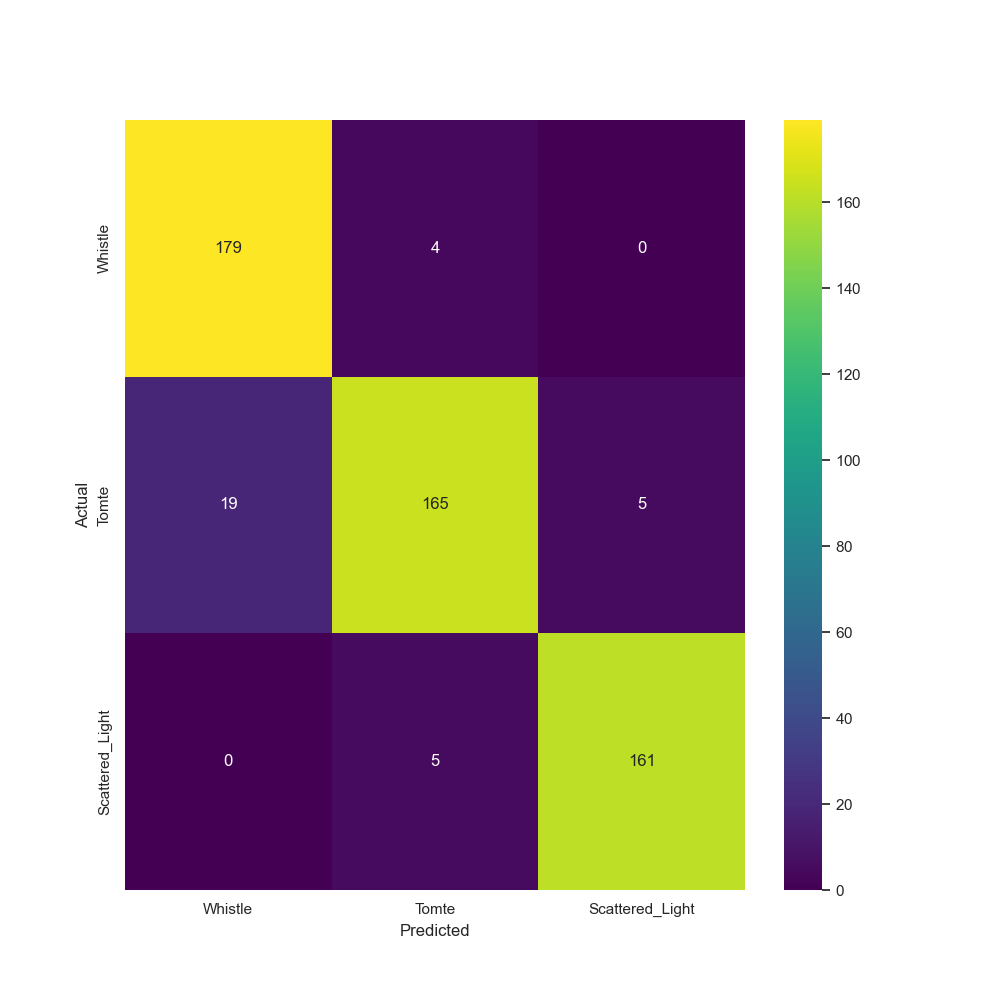
\includegraphics[width=0.45\textwidth]{Images/cm_FD_model_naive.png}  
  \label{fig:fd_sub-first}
\end{subfigure}
\begin{subfigure}
  \centering
  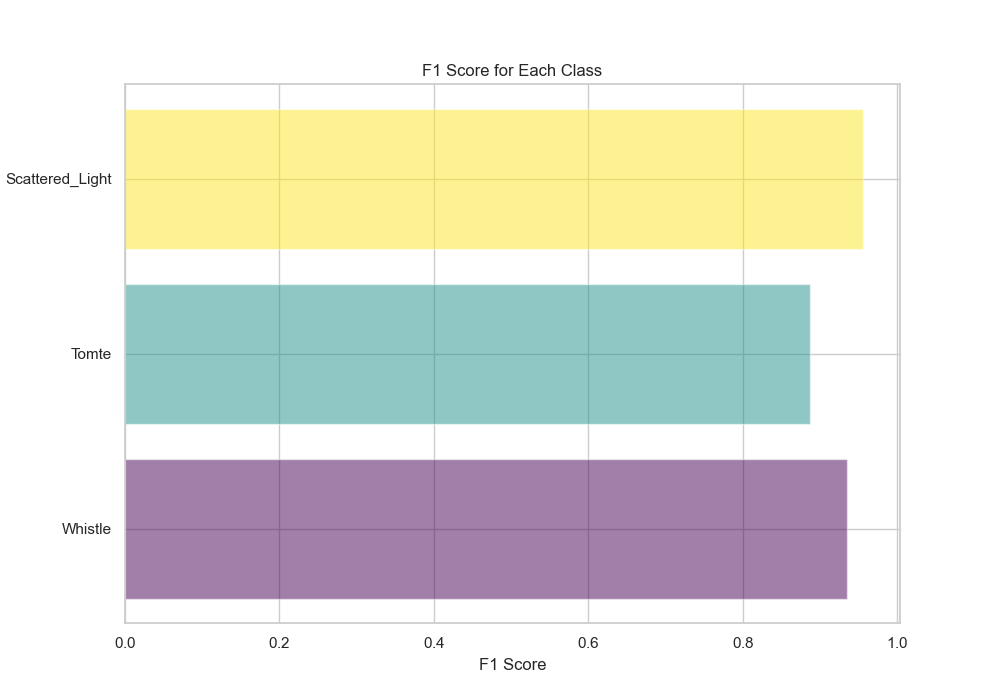
\includegraphics[width=0.50\textwidth]{Images/f1_FD_model_naive.png}  
  \label{fig:fd_sub-second}
\end{subfigure}
\caption{Confusion matrix and f1 plot for Naive baseline}
\label{fig:cm_f1_FD_naive_baseline}
\end{figure}

\begin{table}[ht]
\centering
    \begin{tabular}{|l|c c c|}
    \hline
    \textbf{Glitch type} & \textbf{Precision} & \textbf{Recall} & \textbf{f1-score} \\ \hline
    Whistle & $0.92$ & $0.91$ & $0.92$ \\
    Tomte & $0.87$ & $0.92$ & $0.89$ \\
    Scattered\_Light & $0.98$ & $0.95$ & $0.96$ \\
    \hline
    \end{tabular}
    \caption{Classification report of the FD Naive strategy.}
    \label{tbl:RQ2_class_report_FD_Naive}
\end{table}

Just as in our experiments for \ref{subsec:RQ1} we investigate the \acrshort{tsne} and \acrshort{umap} representations. 
As depicted in Figure \ref{fig:tSNE_FD_Naive}, the t-SNE visualization demonstrates the clustering of three glitch classes in a 2D layout. The plot shows clear separation among the three classes, implying that the model successfully differentiates these glitch types. The compactness of the point clouds within each class suggests high similarity among the data samples of a class. Nonetheless, there is some intersection involving the 'Tomte' class and the other two classes.\\

A similar interpretation can be made from Figure \ref{fig:umap_FD_Naive}. The 'Whistle' class forms a distinct elongated cluster. This indicates that the instances are quite alike in the high-dimensional space. The 'Tomte' cluster appears as a dense group, yet it is proximate to other clusters. It is evident that there is overlap among different classes. This raises the concern whether some instances might have been incorrectly classified during manual labeling. 

\begin{figure}[ht]
  \centering
    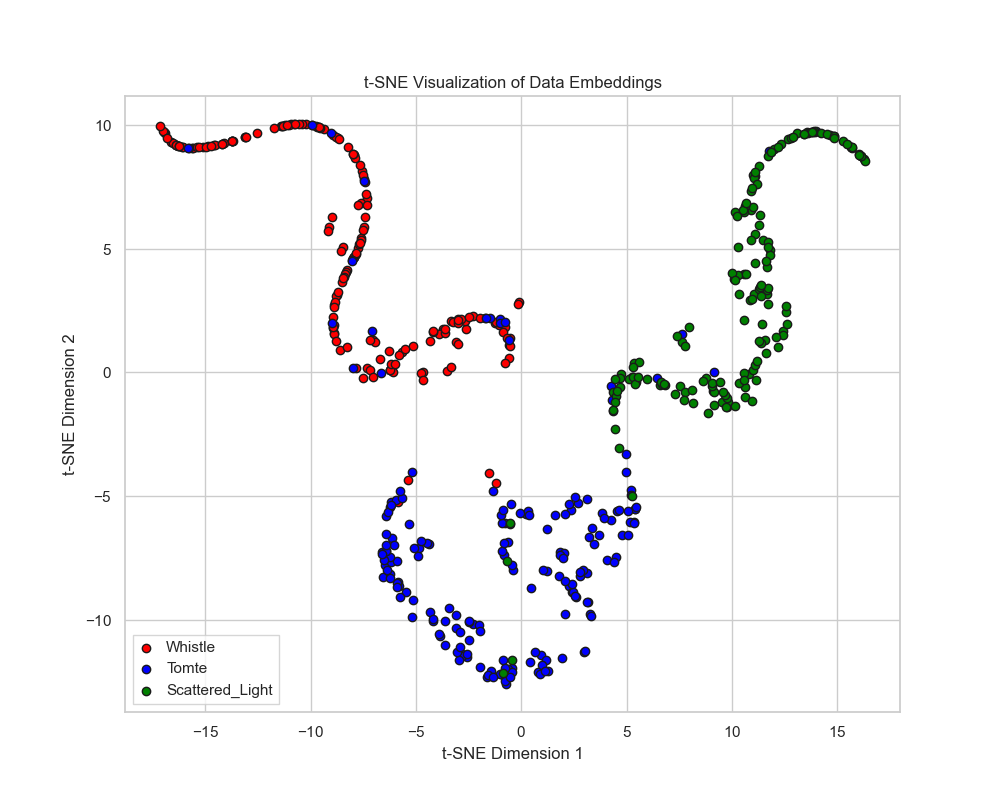
\includegraphics[width=0.9\textwidth]{Grad Assignment/Images/tSNE_FractalDimension_naive_test.png}
    \caption{t-SNE visualization Naive FD strategy}
    \label{fig:tSNE_FD_Naive}
\end{figure}

\begin{figure}[H]
  \centering
    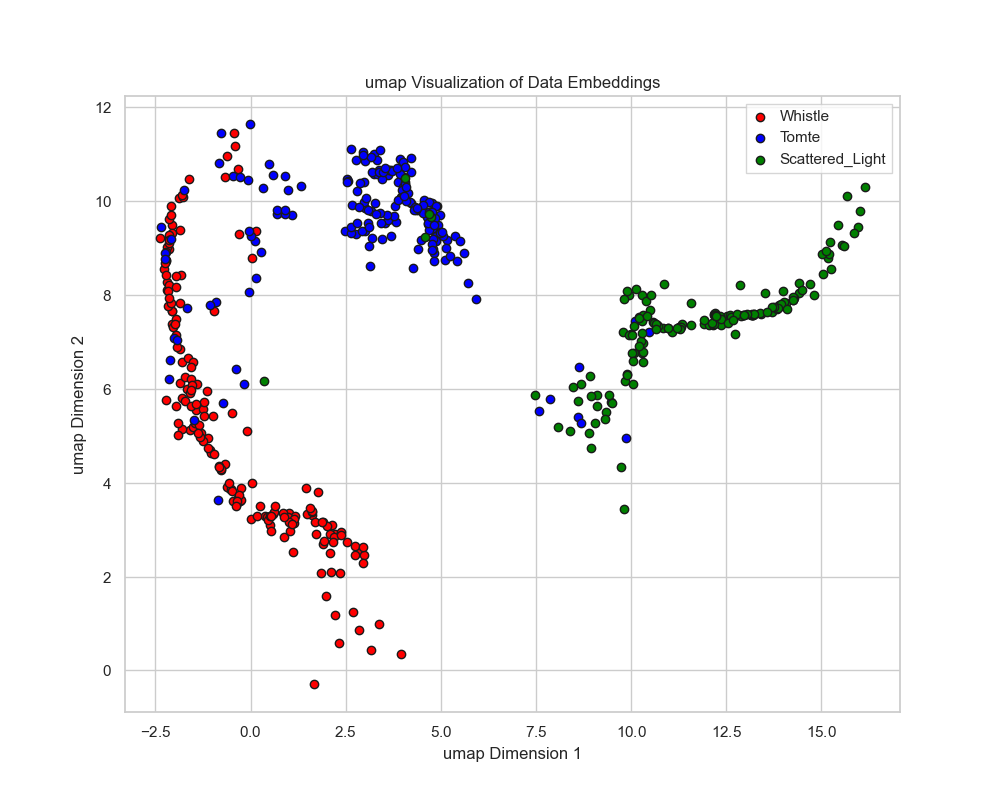
\includegraphics[width=0.9\textwidth]{Grad Assignment/Images/umap_FractalDimension_naive_test.png}
    \caption{UMAP visualization Naive FD strategy}
    \label{fig:umap_FD_Naive}
\end{figure}


\subsubsection{LwF strategy}
\label{subsubsec:RQ2_lwf}
The strategy is implemented with the same hyperparameter choices as described in \ref{subsubsec:RQ1_LWF}. The benchmark as described in \ref{subsubsec:RQ2_naive} is used. \\
The trained model has an overall accuracy of $92\%$, less than the Naive baseline. The F1 scores (see Table \ref{tbl:RQ2_class_report_FD_LwF}) are all less than those of the Naive baseline. 

\begin{figure}[H]
\centering
\begin{subfigure}
  \centering
  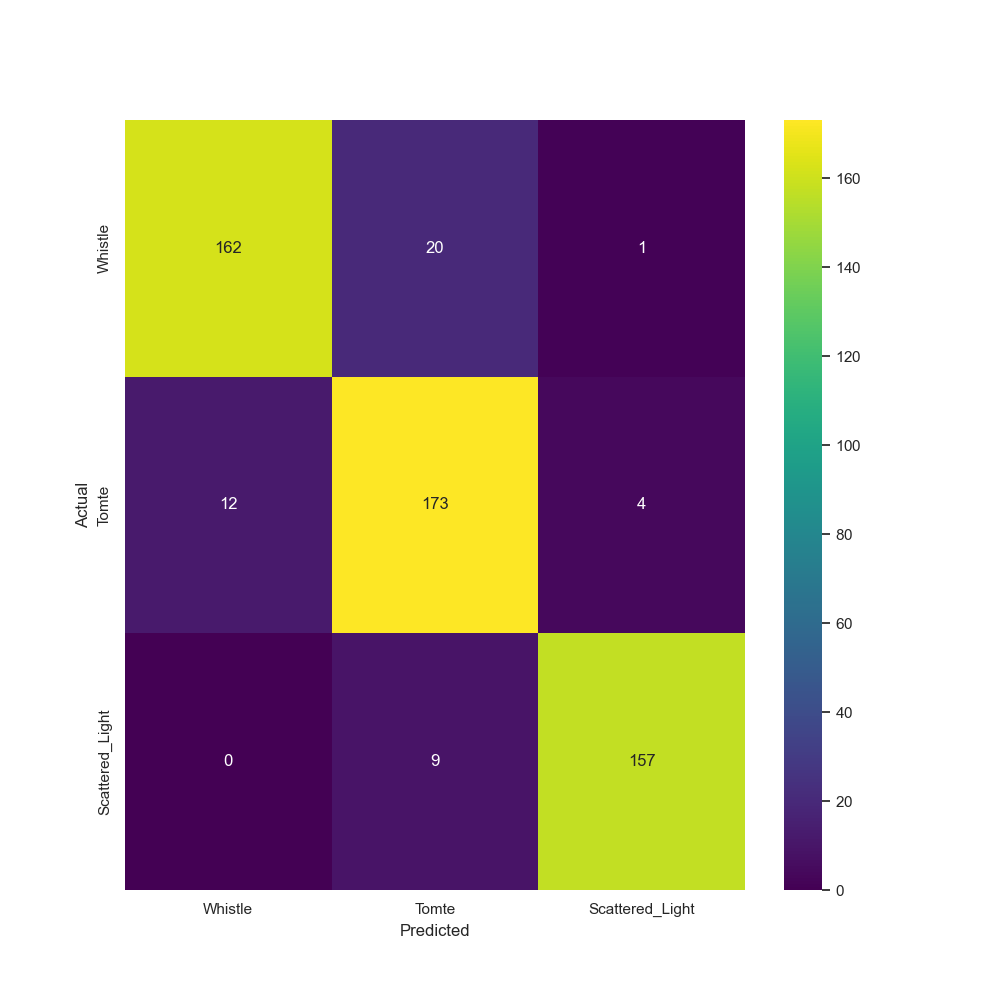
\includegraphics[width=0.45\textwidth]{Images/cm_FD_model_LwF.png}  
  \label{fig:fd_sub-first}
\end{subfigure}
\begin{subfigure}
  \centering
  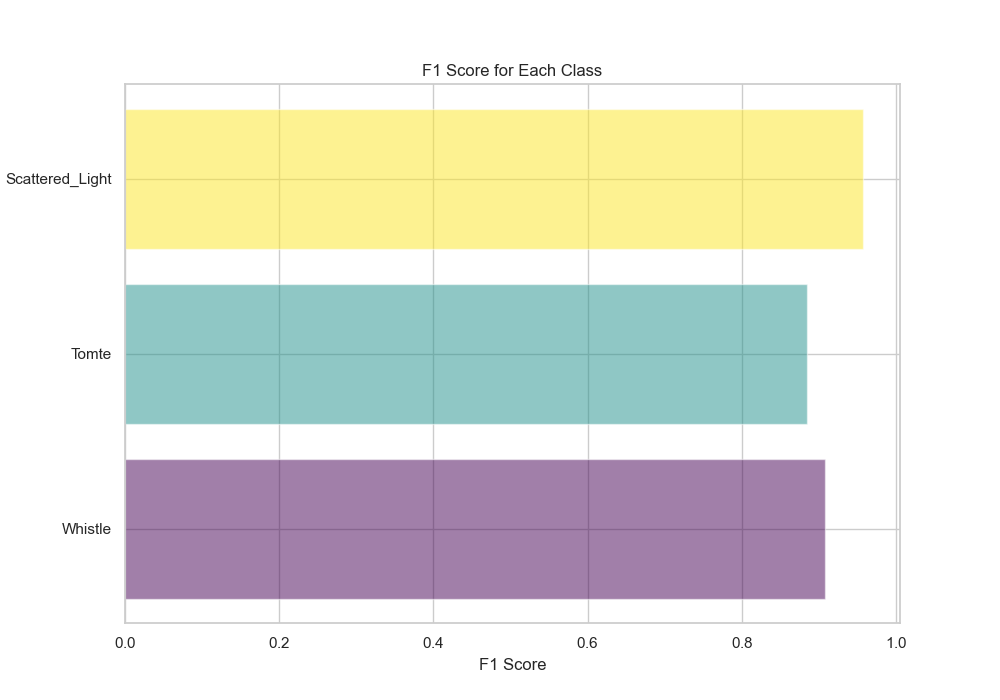
\includegraphics[width=0.50\textwidth]{Images/f1_FD_model_LwF.png}  
  \label{fig:fd_sub-second}
\end{subfigure}
\caption{Confusion matrix and f1 plot for LwF FD strategy}
\label{fig:cm_f1_FD_LwF}
\end{figure}

\begin{table}[ht]
\centering
    \begin{tabular}{|l|c c c|}
    \hline
    \textbf{Glitch type} & \textbf{Precision} & \textbf{Recall} & \textbf{f1-score} \\ \hline
    Whistle & $0.93$ & $0.91$ & $0.92$ \\
    Tomte & $0.87$ & $0.92$ & $0.89$ \\
    Scattered\_Light & $0.98$ & $0.95$ & $0.96$ \\
    \hline
    \end{tabular}
    \caption{Classification report of the FD LwF strategy.}
    \label{tbl:RQ2_class_report_FD_LwF}
\end{table}

The Backward Transfer (BWT) metric is $-0.0654$, suggesting the model had a slight decline in performance on the old task after learning the new task. However, the magnitude of forgetting is relatively small. 

\begin{figure}[!ht]
\centering
\begin{subfigure}
  \centering
    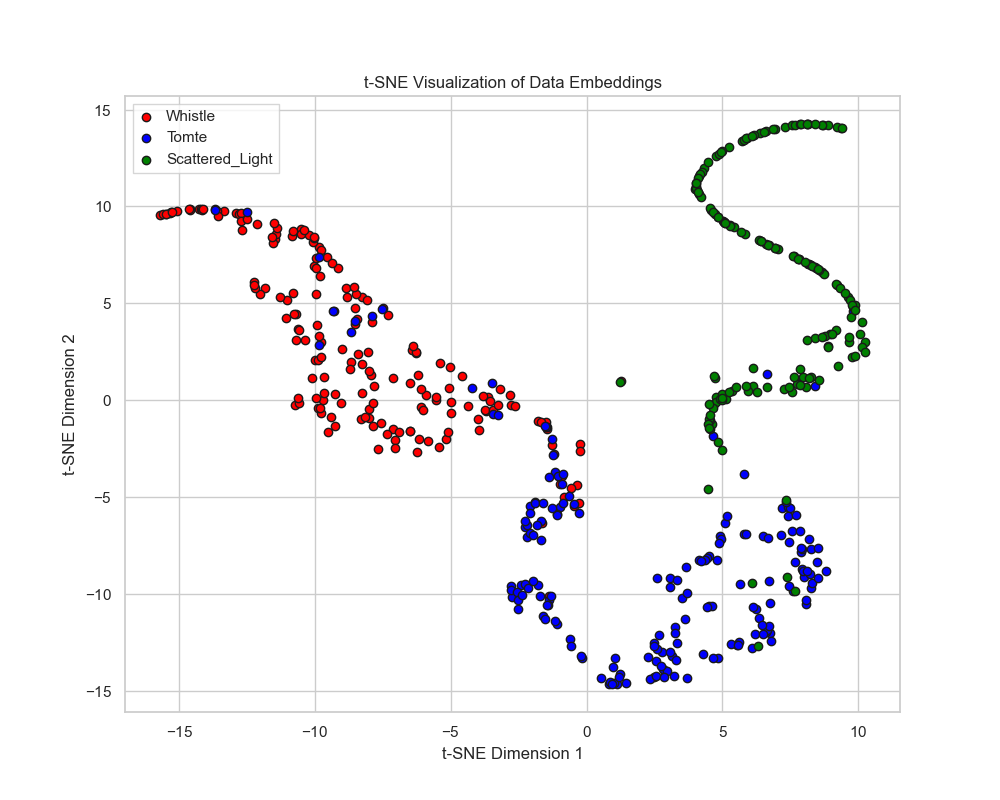
\includegraphics[width=0.7\textwidth]{Images/tSNE_FractalDimension_LwF_test.png}
    \caption{t-SNE visualization LwF FD strategy}
    \label{fig:tSNE_FD_LwF}
\end{subfigure}
\begin{subfigure}
  \centering
    \includegraphics[width=0.7\textwidth]{Images/umap_FractalDimension_LwF_test.png}
    \caption{UMAP visualization LwF FD strategy}
    \label{fig:umap_FD_LwF}
\end{subfigure}
\end{figure}

The 'Scattered\_Light' glitch category has the highest overall F1 score, and from the \acrshort{tsne} and \acrshort{umap} representations shown in Figure \ref{fig:tSNE_FD_LwF} and \ref{fig:umap_FD_LwF} it is clear that the cluster containing the 'Scattered\_Light' test instances is much more dense, as opposed to the 'Whistle' and 'Tomte' clusters showing quite some overlap. This indicates the model has more trouble distinguishing between those two categories. 

\subsubsection{AGEM strategy}
\label{subsubsec:RQ2_agem}
The strategy is augmented, just as in \ref{subsubsec:RQ1_AGEM} with the \verb|ReplayPlugin|, and also an \verb|AGEMPlugin|. The \verb|AGEMPlugin| is set to accept \verb|patterns_per_experience=20|, based on the study by \citep{chaudhry2019continual}. 
The \verb|sample_size| is set to the dataloader size as previously suggested. 
The results, even after retraining with different memory size and patterns\_per\_experience, are very bad. \acrshort{agem} clearly suffers from catastrophic forgetting as depicted in Figure \ref{fig:cm_FD_agem} and it is impossible to plot the \acrshort{tsne} and \acrshort{umap} plots because of \verb|nan| values occurring in the loss calculation. 
The model outputs the last encountered class 'Whistle' in all test cases. 
\begin{figure}[H]
    \centering
    \includegraphics[width=0.6\textwidth]{Grad Assignment/Images/cm_FD_model_AGEM.png}
    \caption{Confusion matrix for AGEM strategy}
    \label{fig:cm_FD_agem}
\end{figure}


\subsubsection{EWC strategy}
\label{subsubsec:RQ2_ewc}
The strategy is implemented with the same hyperparameter choices as described in \ref{subsubsec:RQ1_EWC}. The benchmark as described in \ref{subsubsec:RQ2_naive} is used. \\
The trained model has an overall accuracy of $90\%$, less than the Naive baseline. The F1 scores (see Table \ref{tbl:RQ2_class_report_FD_EWC}) are all less than those of the Naive baseline. 

\begin{figure}[!ht]
\centering
\begin{subfigure}
  \centering
  \includegraphics[width=0.45\textwidth]{Images/cm_FD_model_EWC.png}  
  \label{fig:fd_sub-first}
\end{subfigure}
\begin{subfigure}
  \centering
  \includegraphics[width=0.50\textwidth]{Images/f1_FD_model_EWC.png}  
  \label{fig:fd_sub-second}
\end{subfigure}
\caption{Confusion matrix and f1 plot for EWC FD strategy}
\label{fig:cm_f1_FD_EWC}
\end{figure}

\begin{table}[!ht]
\centering
    \begin{tabular}{|l|c c c|}
    \hline
    \textbf{Glitch type} & \textbf{Precision} & \textbf{Recall} & \textbf{f1-score} \\ \hline
    Whistle & $0.89$ & $0.93$ & $0.91$ \\
    Tomte & $0.85$ & $0.87$ & $0.86$ \\
    Scattered\_Light & $0.97$ & $0.90$ & $0.94$ \\
    \hline
    \end{tabular}
    \caption{Classification report of the FD EWC strategy.}
    \label{tbl:RQ2_class_report_FD_EWC}
\end{table}

The Backward Transfer (BWT) metric is $-0.1176$, suggesting a moderate level of catastrophic forgetting on the previous experiences after learning the new experience.

\subsubsection{DER strategy}
\label{subsubsec:RQ2_der}
The strategy is implemented with the same hyperparameter choices as described in \ref{subsubsec:RQ1_DER} with the benchmark as described in \ref{subsubsec:RQ2_naive}. \\
The trained model has an overall accuracy of $90\%$, less than the Naive baseline. The F1 scores (see Table \ref{tbl:RQ2_class_report_FD_EWC}) are all less than those of the Naive baseline. 

\begin{figure}[!ht]
\centering
\begin{subfigure}
  \centering
  \includegraphics[width=0.45\textwidth]{Images/cm_FD_model_DER.png}  
  \label{fig:fd_sub-first8}
\end{subfigure}
\begin{subfigure}
  \centering
  \includegraphics[width=0.50\textwidth]{Images/f1_FD_model_DER.png}  
  \label{fig:fd_sub-second8}
\end{subfigure}
\caption{Confusion matrix and f1 plot for DER FD strategy}
\label{fig:cm_f1_FD_DER}
\end{figure}

\begin{table}[ht]
\centering
    \begin{tabular}{|l|c c c|}
    \hline
    \textbf{Glitch type} & \textbf{Precision} & \textbf{Recall} & \textbf{f1-score} \\ \hline
    Whistle & $0.89$ & $0.93$ & $0.91$ \\
    Tomte & $0.85$ & $0.87$ & $0.86$ \\
    Scattered\_Light & $0.97$ & $0.90$ & $0.94$ \\
    \hline
    \end{tabular}
    \caption{Classification report of the FD DER strategy.}
    \label{tbl:RQ2_class_report_FD_DER}
\end{table}

The Backward Transfer (BWT) metric is $0.0131$, indicating that the model was successful in mitigating forgetting on the old task while the model learned the new task. A BWT close to zero (ideal scenario) indicates that the model is able to maintain its performance on old tasks while learning new ones with no degradation in performance on old tasks.


\subsubsection{DER++ strategy}
\label{subsubsec:RQ2_der++}
The strategy is implemented with the identical hyperparameter values as described in \ref{subsubsec:RQ1_DER++} with the benchmark as described in \ref{subsubsec:RQ2_naive}. \\
The trained model has an overall accuracy of $77\%$, this is the worst performing model. The F1 scores (see Table \ref{tbl:RQ2_class_report_FD_DER++}) are all less than those of the Naive baseline. Especially very bad performance metrics on the 'Tomte' glitch. 
\begin{figure}[!ht]
\centering
\begin{subfigure}
  \centering
  \includegraphics[width=0.45\textwidth]{Images/cm_FD_model_DER++.png}  
  \label{fig:fd_sub-first}
\end{subfigure}
\begin{subfigure}
  \centering
  \includegraphics[width=0.50\textwidth]{Images/f1_FD_model_DER++.png}  
  \label{fig:fd_sub-second}
\end{subfigure}
\caption{Confusion matrix and f1 plot for DER++ FD strategy}
\label{fig:cm_f1_FD_DER++}
\end{figure}

\begin{table}[ht]
\centering
    \begin{tabular}{|l|c c c|}
    \hline
    \textbf{Glitch type} & \textbf{Precision} & \textbf{Recall} & \textbf{f1-score} \\ \hline
    Whistle & $0.80$ & $1.00$ & $0.89$ \\
    Tomte & $0.96$ & $0.36$ & $0.52$ \\
    Scattered\_Light & $0.68$ & $0.98$ & $0.81$ \\
    \hline
    \end{tabular}
    \caption{Classification report of the FD DER++ strategy.}
    \label{tbl:RQ2_class_report_FD_DER++}
\end{table}

The Backward Transfer (BWT) metric is $-0.0458$, suggesting the model had a slight decline in performance on the old task after learning the new task. However, the magnitude of forgetting is relatively small. 

The \acrshort{tsne} plot in \ref{fig:tsne_FD_DER++} illustrates the difficulty of differentiating between 'Tomte' and the other two classes. 

\begin{figure}[H]
    \centering
    \includegraphics[width=0.7\textwidth]{Grad Assignment/Images/tSNE_FractalDimension_DER++_test.png}
    \caption{t-SNE visualization DER++ FD strategy}
    \label{fig:tsne_FD_DER++}
\end{figure}


\subsubsection{SCR strategy}
\label{subsubsec:RQ2_scr}
The \acrshort{scr} stategy on the Fractal Dimension data has a similar implementation as in \ref{subsub:RQ1_SCR}. The model has an overall accuracy of $93\%$ and scores second just after the Naive strategy used in \ref{subsubsec:RQ2_naive}. 
The weight distributions shown in Figure \ref{tbl:scr_fd_weights} indicate the difficulty the model has with distinguishing 'Whistle' and 'Tomte' glitches. Behavior that is confirmed by the \acrshort{tsne} and \acrshort{umap} plots in Figures \ref{fig:tsne_FD_SCR} and \ref{fig:umap_FD_SCR}. 
\begin{center}
\begin{tabular}{cc}
\includegraphics[width=0.4\textwidth]{Images/SCR_MultiView_exp_0.png} & \includegraphics[width=0.4\textwidth]{Images/SCR_MultiView_exp_2.png} \\
\end{tabular}
\label{tbl:scr_fd_weights}
\end{center}
The Backward Transfer (BWT) metric is $0.3595$, a high value, suggesting that the model suffers from moderate catastrophic forgetting on the old task after learning the new task.  

\begin{table}[ht]
\centering
    \begin{tabular}{|l|c c c|}
    \hline
    \textbf{Glitch type} & \textbf{Precision} & \textbf{Recall} & \textbf{f1-score} \\ \hline
    Whistle & $0.94$ & $0.96$ & $0.95$ \\
    Tomte & $0.93$ & $0.85$ & $0.89$ \\
    Scattered\_Light & $0.91$ & $0.96$ & $0.94$ \\
    \hline
    \end{tabular}
    \caption{Classification report of the FD SCR strategy.}
    \label{tbl:RQ2_class_report_FD_SCR}
\end{table}

\begin{figure}[H]
    \centering
    \includegraphics[width=0.7\textwidth]{Images/tSNE_FractalDimension_SCR_test.png}
    \caption{t-SNE visualization SCR FD strategy}
    \label{fig:tsne_FD_SCR}
\end{figure}

\begin{figure}[H]
    \centering
    \includegraphics[width=0.7\textwidth]{Images/umap_FractalDimension_SCR_test.png}
    \caption{UMAP visualization SCR FD strategy}
    \label{fig:umap_FD_SCR}
\end{figure}
\newpage

\subsection{RQ3}
\label{subsub:rq3}
The training is done on the dataset provided by Melissa Lopez, used in the research by \citep{laguarta2023detection, dooney2022dvgan, dooney2024cdvgan}. The training is done for 30 epochs on the classes \{Whistle, Scattered\_Light, Tomte\}. 

The ultimate version of the model achieved a Cross Entropy Loss of $0.0122$ and a training accuracy of $99.61\%$. The outcomes detailed in \ref{tbl:RQ3_class_report_multimodal} for the unseen test samples were remarkably impressive, demonstrating flawless precision, recall, and f1-score across all three categories. Notably, the performance on the Tomte glitch significantly surpassed that of earlier 'best' models as discussed in \ref{subsubsec:RQ1_DER} and \ref{subsubsec:RQ2_naive}.

\begin{table}[ht]
\centering
    \begin{tabular}{|l|c c c|}
    \hline
    \textbf{Glitch type} & \textbf{Precision} & \textbf{Recall} & \textbf{f1-score} \\ \hline
    Whistle & $1.00$ & $1.00$ & $1.00$ \\
    Tomte & $1.00$ & $1.00$ & $1.00$ \\
    Scattered\_Light & $1.00$ & $1.00$ & $1.00$ \\
    \hline
    \end{tabular}
    \caption{Classification report of the Multimodal architecture.}
    \label{tbl:RQ3_class_report_multimodal}
\end{table}

The resulting \acrshort{tsne} plot confirms the perfect test set results. There are two points that may be outliers or incorrectly classified by the Gravity Spy project \citep{zevin2017gravity}. 

\begin{figure}[H]
    \centering
    \includegraphics[width=0.9\textwidth]{Grad Assignment/Images/tSNE_RQ3_ImageModel_test.png}
    \caption{t-SNE visualization of Multimodal architecture.}
    \label{fig:tsne_multimodal}
\end{figure}
\newpage
The Saliency mapping in Figure \ref{fig:saliency_mapping_multimodal} illustrates the distinctive capabilities of the model. There are clear boundaries between the three glitch categories. 
\begin{figure}[H]
    \centering
    \includegraphics[width=1.0\textwidth]{Grad Assignment/Images/SaliencyMapping_Multimodal_test.png}
    \caption{Saliency mapping of the Multimodal architecture.}
    \label{fig:saliency_mapping_multimodal}
\end{figure}
